\documentclass[]{sfuthesis}

\usepackage[english]{babel}             % ensure USenglish hyphenation
\usepackage[T1]{fontenc}                % copyable accent characters (e.g. ö)
% \usepackage[utf8]{inputenc}             % included by default since 2018
% \usepackage{textcomp}                   % included by default since 2020

\PassOptionsToPackage{hyphens}{url}

% Load before most packages https://tex.stackexchange.com/a/26592/2930
\usepackage[
  hidelinks,                            % remove colored boxes around links
  pdfusetitle,                          % use \title and \author for PDF metadata
  colorlinks,                           % color links instead of boxes (like CVPR)
  linkcolor=black,                      % color of internal links
]{hyperref}

% Bibliography
\usepackage[
  style=ieee,
  backref=true,
  backrefstyle=none,
]{biblatex}

\usepackage{amssymb}
\usepackage[titletoc]{appendix}
\usepackage{booktabs}                   % \toprule, \midrule, \bottomrule
\usepackage[font=small, skip=12pt, labelfont=bf]{caption}
\usepackage[inline]{enumitem}           % Advanced enumerate and itemize.
\usepackage{float}                      % \begin{figure}[H]
\usepackage{geometry}
\usepackage{graphicx}
\usepackage{grffile}                    % graphicx filename extensions
\usepackage{import}                     % \import
\usepackage{makecell}                   % \makecell in tables
\usepackage{makecmds}                   % \provideenvironment
\usepackage{mathtools}
\usepackage{microtype}                  % improves spacing between words and letters
\usepackage{multirow}                   % \multirow, \multicolumn for tables
\usepackage{placeins}                   % \FloatBarrier
\usepackage{setspace}                   % \onehalfspacing
\usepackage{silence}                    % \WarningFilter
\usepackage{standalone}
\usepackage{subcaption}                 % \begin{subfigure}
\usepackage{tabularx}                   % \begin{tabularx}
\usepackage{titlesec}                   % improves spacing between section headings
\usepackage{threeparttable}             % \begin{tablenotes}
\usepackage{xcolor}                     % \textcolor

\usepackage{lmodern}                    % font: Latin Modern
% \usepackage{unicode-math}               % font: Latin Modern Math (XeTeX/LuaTeX)
% \usepackage{newpxtext,newpxmath}        % font: Palatino
\usepackage{newtxtext}                  % font: Times
% \usepackage{newtxmath}                  % font: Times Math

\usepackage[outputdir=out]{minted}      % code highlighting

% % Load subcaption with compatibility with IEEEtran:
% % https://tex.stackexchange.com/questions/154435/ieee-template-and-caption-false-option-for-subcaption-package
% \makeatletter
% \let\MYcaption\@makecaption
% \makeatother
% \WarningFilter*{caption}{Unknown document class (or package)}
% \usepackage[font=footnotesize]{subcaption}
% \makeatletter
% \let\@makecaption\MYcaption
% \makeatother

% Load after minted/fvextra
\usepackage{csquotes}

% % Load after xcolor
% \usepackage{tikz}

% Load after subcaption
\usepackage{alphalph}

% Load after amsmath
\usepackage[
  capitalize,
  nameinlink,
  % noabbrev,
]{cleveref}

% No "Eq." prefix
\crefname{equation}{}{}

% Abstract for book documentclass
\provideenvironment{abstract}{}{}
\usepackage{abstract}


% Chapter abstracts
% See also:
% https://tex.stackexchange.com/questions/309072/how-to-add-abstract-for-selected-chapters-in-my-thesis
% https://tex.stackexchange.com/questions/377893/configure-the-abstract-at-a-chapter-of-thesis-in-the-same-page-with-chapters-ti
\newenvironment{chapabstract}{%
  % \begin{quote}%
  %   \small \rule{14cm}{1pt}%
  \begin{list}{}{%
    \setlength{\leftmargin}{12.5mm}%
    \setlength{\rightmargin}{\leftmargin}%
  }%
  \item%
    \begin{center}%
      \rule{\linewidth}{1pt}%
      \vspace*{-0.5ex+1ex}
      \large \bfseries Abstract
      \vspace{-.5em} \vspace{0pt}
    \end{center}
  \item\relax%
}{%
  \par%
  \vspace{-\baselineskip+1ex+1ex}%
  \rule{\linewidth}{1pt}%
  \end{list}%
  \vspace{1ex}%
  %   \vskip-4mm\rule{14cm}{1pt}%
  % \end{quote}%
}


% References
\addbibresource{references/cfm.bib}
\addbibresource{references/compression.bib}
\addbibresource{references/imagecompression.bib}
\addbibresource{references/misc.bib}
\addbibresource{references/pointcloud.bib}
\addbibresource{references/pointcloudcompression.bib}


% Do not print DOI if URL or eprint is present.
% https://tex.stackexchange.com/questions/29802/biblatex-and-new-line-for-doi-url-and-eprint
\renewbibmacro*{doi+eprint+url}{%
  \iftoggle{bbx:doi}
    {\iffieldundef{url}{\iffieldundef{eprint}{\printfield{doi}}{}}}
    {}%
  \newunit\newblock
  \iftoggle{bbx:eprint}
    {\usebibmacro{eprint}}
    {}%
  \newunit\newblock
  \iftoggle{bbx:url}
    {\usebibmacro{url+urldate}}
    {}}


% % TikZ libraries
% \usetikzlibrary{
%   external,
% }

% Code listing style
\usemintedstyle{pastie}


% Suppress warnings
\pdfsuppresswarningpagegroup=1

% Keep footnotes on one page
\interfootnotelinepenalty=10000

% Page margins
\newgeometry{
  top=1in,
  left=1.25in,
  bottom=0.7in,
  right=1.25in,
  includefoot
}

% Line spacing
\onehalfspacing

% Empty header; page number in footer
\pagestyle{plain}

% Automatically style inner and outer quotation marks
\MakeOuterQuote{"}

% Citation style
\DeclareFieldFormat{title}{\mkbibquote{#1}}


% Code listing
\newif\ifhighlightcode
\highlightcodetrue

\makeatletter
\ifhighlightcode%
  \let\codelisting\minted
  \let\endcodelisting\endminted
\else%
  \newenvironment{codelisting}[2][]{%
    \VerbatimEnvironment
    \begin{Verbatim}%
  }{%
    \end{Verbatim}%
    \ignorespacesafterend%
  }%
\fi
\makeatother


\DeclareMathOperator{\E}{\mathbb{E}}
\DeclareMathOperator{\sign}{sign}
\DeclareMathOperator*{\argmax}{arg\,max}
\DeclareMathOperator*{\argmin}{arg\,min}
\newcommand{\boldvar}[1]{{\boldsymbol{#1}}}


% https://tex.stackexchange.com/questions/78098/captioning-nested-subfigures-with-subcaption/689184#689184
\newenvironment{subsubfigure}[2][]{%
  \begin{subfigure}[#1]{#2}%
    \stepcounter{subsubfigure}%
    \renewcommand{\thesubfigure}{\roman{subsubfigure}}%
}{%
    \addtocounter{subfigure}{-1}%
  \end{subfigure}%
}
\newcounter{subsubfigure}


\newlength{\tablesepskip}
\newlength{\tablesubheaderskip}


% \tikzexternalize[prefix=out/]

\title{Learned Compression for Images and Point Clouds}
\author{Mateen Ulhaq}
\date{today}

\thesistype{Thesis}
\previousdegrees{}
\degree{Master of Applied Science}
\discipline{Engineering}
\department{School of Engineering Science}
\faculty{Faculty of Applied Sciences}
\copyrightyear{2023}
\semester{Summer 2023}

\keywords{%
  deep learning;
  compression;
  inference%
}

\committee{%
  \chair{Dr. Ivan V. Baji\'c, P.Eng.}{Academic Supervisor \\ Professor}
  % \member{Dr. Mirza Faisal Beg, P.Eng.}{Committee \\ Professor}
  % \member{Dr. Jie Liang, P.Eng.}{Committee \\ Professor}
}

\includeonly{
  tex/abstract,
  % tex/acknowledgments,
  % tex/introduction/init,
  tex/point_cloud/init,
  % tex/conclusion/init,
}

\begin{document}

\frontmatter

\maketitle
\makecommittee
\clearpage
% \phantomsection
% \addcontentsline{toc}{chapter}{Abstract}
\newcounter{abstractpage}
\setcounter{abstractpage}{\value{page}}

\begin{abstract}
  \thispagestyle{plain}
  \setcounter{page}{\value{abstractpage}}

  TODO

  \setcounter{abstractpage}{\value{page}}
\end{abstract}

\setcounter{page}{\value{abstractpage}}
\stepcounter{page}

\chapter*{Acknowledgments}
\addcontentsline{toc}{chapter}{Acknowledgements}

Under construction.


% Ivan V. Baji\'c, P.Eng. for his guidance and support throughout my graduate studies.
%
% Committee members
%
% Interdigital for the internship opportunity.
% In particular, my immediate team members:
% Hyomin Choi
% Fabien Racap\'e
% Ujwal Dinesha and Ezgi Ozyilkan
%
% Alon Harell
% Anderson de Andrade
%
% Family, friends



\clearpage
\phantomsection
\pdfbookmark{\contentsname}{toc}
\tableofcontents
\listoffigures

\clearpage
\pagenumbering{arabic}

\mainmatter

% https://tex.stackexchange.com/questions/1989/speed-up-compilation-by-pre-compiling-chapters-separately
% https://tex.stackexchange.com/questions/246/when-should-i-use-input-vs-include
%
% Use \include for each chapter.
% Use \input for each section.

\chapter{Introduction}
\label{chap:introduction}

\IfFileExists{tex/introduction/wip.tex}{%
  \input{tex/introduction/wip.tex}%
}{%
  Under construction.
  % \typeout{Warning: Missing file tex/introduction/wip.tex}%
}

\begin{itemize}
  \item Motivation
  \item Compression (briefly: Shannon, lossy, lossless, arithmetic coding)
  \item VAEs (briefly)
  \item Ballé~\emph{et~al.}~\cite{balle2018variational}
  \item How entropy models work
  \item Entropy bottleneck
  \item Gaussian conditional
  \item Transform architecture notation ($g_a$, $g_s$)
  \item More advanced learned entropy models
  \item Other related work, background knowledge
\end{itemize}


\chapter{Latent space motion analysis for collaborative intelligence}
% \chapter{Latent Space Motion Analysis for Collaborative Intelligence}
\label{ch:video_latent_space_motion_analysis}

% Changes made:
%
% Replacements:
% :%s/eq:/eq:video_latent_space_motion_analysis\//g
% :%s/fig:/fig:video_latent_space_motion_analysis\//g
% :%s/sec:/sec:video_latent_space_motion_analysis\//g
% :%s/img\//img\/video_latent_space_motion_analysis\//g
% :%s/Duan2020VideoCF/duan2020vcm/g
% :%s/Choi2018NearLosslessDF/choi2018mmsp/g
%
% Removals:
% \vspace{...}
% \FloatBarrier
%
% Reorder:
% figures




% \usepackage{flushend}
% \usepackage{fancyhdr}
% \pagestyle{fancy}
% \fancyhf{}
% \renewcommand{\headrulewidth}{0pt}% Header rule
% \renewcommand{\footrulewidth}{0pt}% Footer rule
% \fancyhead[C]{}
%
% \fancypagestyle{firstpage}{% Page style for first page
%   \fancyhf{}% Clear header/footer
%   \renewcommand{\headrulewidth}{0pt}% Header rule
%   \renewcommand{\footrulewidth}{0pt}% Footer rule
%   \fancyhead[C]{\vspace{-2.2cm}Extended version of the paper ``Latent Space Motion Analysis for Collaborative Intelligence,'' to be presented at the IEEE International Conference on Acoustics, Speech and Signal Processing (ICASSP), Toronto, Canada, June 6-1, 2021. \vspace{0.3cm}}
% }




\begin{center}
  \small
  Notice: This chapter has been reproduced from the paper~\cite{ulhaq2021analysis}.
\end{center}




\begin{chapabstract}
When the input to a deep neural network (DNN) is a video signal, a sequence of feature tensors is produced at the intermediate layers of the model. If neighboring frames of the input video are related through motion, a natural question is, ``what is the relationship between the corresponding feature tensors?'' By analyzing the effect of common DNN operations on optical flow, we show that the motion present in each channel of a feature tensor is approximately equal to the scaled version of the input motion. The analysis is validated through experiments utilizing common motion models. %These results will be useful in collaborative intelligence applications where sequences of feature tensors need to be compressed or further analyzed.
\end{chapabstract}


% \begin{keywords}
% Collaborative intelligence, latent space motion, feature domain motion, feature compression
% \end{keywords}




\section{Introduction}

Collaborative intelligence (CI)~\cite{Bajic_etal_ICASSP21} has emerged as a promising strategy to bring AI ``to the edge.'' In a typical CI system (\cref{fig:video_latent_space_motion_analysis/CI_system}), a deep neural network (DNN) is split into two parts: the edge sub-model, deployed on the edge device near the sensor, and the cloud sub-model deployed in the cloud. Intermediate features produced by the edge sub-model are transferred from the edge device to the cloud. It has been shown that such a strategy may provide better energy efficiency~\cite{kang2017neurosurgeon,jointdnn}, lower latency~\cite{kang2017neurosurgeon,jointdnn,ulhaq2019neurips_demo}, and lower bitrates over the communication channel~\cite{dfc_for_collab_object_detection,choi2018mmsp}, compared to more traditional cloud-based analytics where the input signal is directly sent to the cloud. These potential benefits will find a number of applications in areas such as intelligent sensing~\cite{Chen19} and video coding for machines~\cite{MPEG_VCM_CFE,duan2020vcm}. In particular, compression of intermediate features has become an important research problem, with a number of recent developments~\cite{Saeed_ICIP19,Hyomin_ICASSP20,Saeed_ICASSP20,Bob_ICME20, Saeed2020pareto_arxiv} for the case when the input to the edge sub-model is a still image.

When the input to the edge sub-model is video, its output is a sequence of feature tensors produced from successive frames in the input video. This sequence of feature tensors needs to be compressed prior to transmission and then decoded in the cloud for further processing. Since motion plays such an important role in video processing and compression, we are motivated to examine whether any similar relationship exists in the latent space among the feature tensors. Our theoretical and experimental results show that, indeed, motion from the input video is approximately preserved in the channels of the feature tensor. %\textcolor{blue}{
An illustration of this is presented in \cref{fig:video_latent_space_motion_analysis/mv_overview}, where the estimated input-space motion field is shown on the left, and the estimated motion fields in several feature tensor channels are shown on the right.
%}
These findings suggest that methods for motion estimation, compensation, and analysis that have been developed for conventional video processing and compression may provide a solid starting point for equivalent operations in the latent space.

\begin{figure}[htbp]
    \centering
    \vspace{\baselineskip}%
    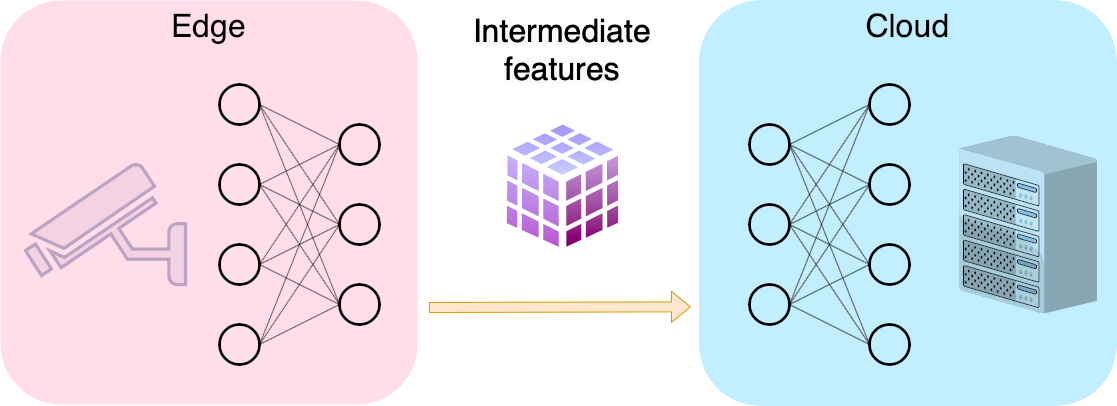
\includegraphics[width=\columnwidth]{img/video_latent_space_motion_analysis/CI_system.png}%
    \vspace{0.5\baselineskip}%
    \caption{Basic collaborative intelligence system.}
    \label{fig:video_latent_space_motion_analysis/CI_system}
    % \vspace{-1.0\baselineskip}
\end{figure}

\begin{figure}[htbp]
    \centering
    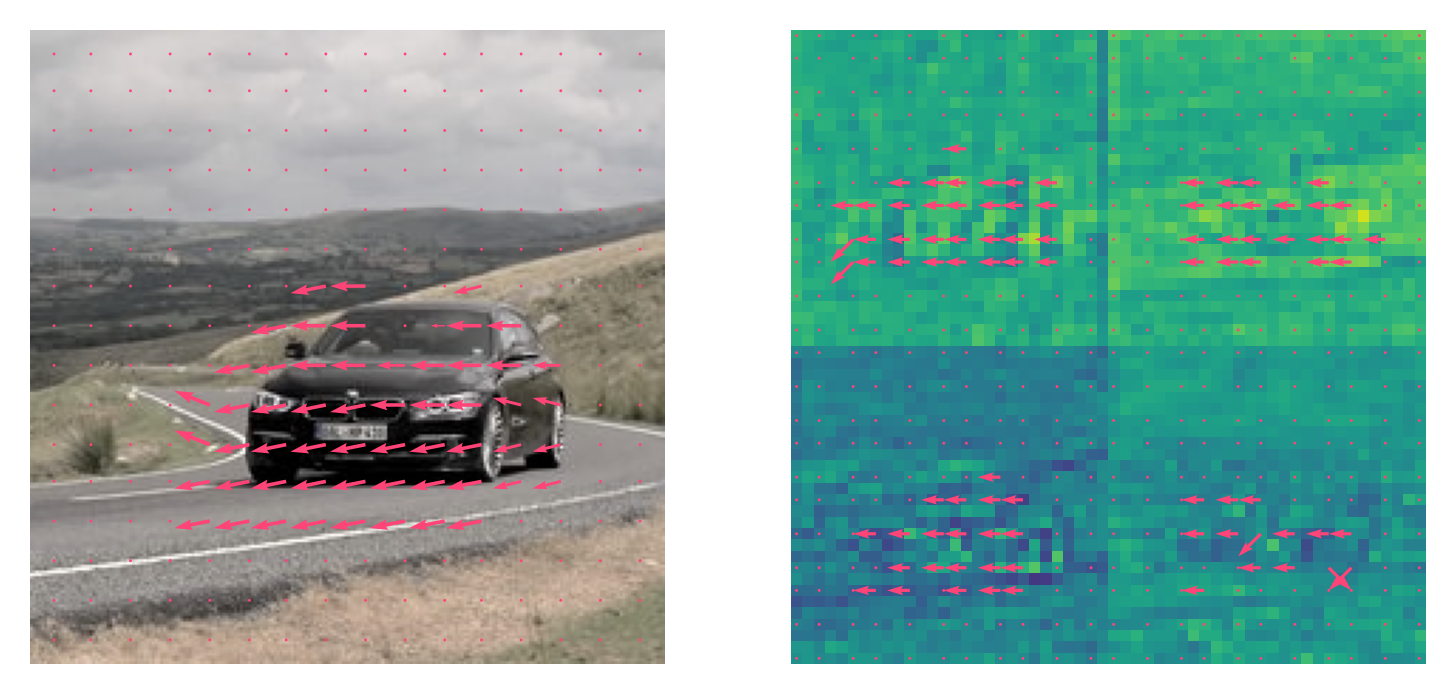
\includegraphics[width=\columnwidth]{img/video_latent_space_motion_analysis/mv_car.png}
    \caption{%
        Motion estimates for input frames (left) and
        select channels from the output of ResNet-34's add\_3 layer (right).
    }
    \label{fig:video_latent_space_motion_analysis/mv_overview}
    % \vspace{-1.0\baselineskip}
\end{figure}

The paper is organized as follows. In \cref{sec:video_latent_space_motion_analysis/motion_analysis}, we analyze the actions of typical operations found in deep convolutional neural networks on optical flow in the input signal, and show that these operations tend to preserve the optical flow, at least approximately, with an appropriate scale. In \cref{sec:video_latent_space_motion_analysis/experiments} we provide empirical support for the theoretical analysis from \cref{sec:video_latent_space_motion_analysis/motion_analysis}. %using canonical motions such as translation, rotation, and scale change.
Finally, \cref{sec:video_latent_space_motion_analysis/conclusions} concludes the paper.


% \FloatBarrier


%The problem may be formulated as follows: Let $x$ be an input frame and $y = f(x)$ be its corresponding output at an intermediate layer within the deep model. Let $x'$ be another input frame that may be related to $x$ by a transformation $x' \approx g(x)$. Provided only $y$ and $g$, can we reliably predict the output $y' = f(x')$?

%For simplicity, assume that the intermediate layer operation is a 2x2 max pool of stride 2. Then in the case of simple translation of the contents of the input frame by $(u, v)$, we may state:

%\[x'_{i, j} = (g_{u, v}(x))_{i, j} = x_{i - u, j - v}\]

%\[y'_{i, j} = y_{i - \sfrac{u}{2}, j - \sfrac{v}{2}}\]

%More generally, for an affine transformation $A(M, u, v)$ (comprised of a linear transformation $M$ and translation $(u, v)$), we may state:

% TODO simplify notation

%\[x'_{i, j} = (g_{u, v}(x))_{i, j} = x_{A^{-1}(M, u, v)(i, j)}\]

%\[y'_{i, j} = y_{A^{-1}(M, \sfrac{u}{2}, \sfrac{v}{2})(i, j)}\]





\section{Latent space motion analysis}
\label{sec:video_latent_space_motion_analysis/motion_analysis}

The basic problem studied in this paper is illustrated in \cref{fig:video_latent_space_motion_analysis/overview}. Consider two images (video frames) input to the edge sub-model of a CI system. It is common to represent their relationship via a motion model. The question we seek to answer here is, ``what is the relationship between the corresponding feature tensors produced by the edge sub-model?'' To answer this question, we will look at the processing pipeline between the input image and a given channel of a feature tensor. In most deep models for computer vision applications, this processing pipeline consists of a sequence of basic operations: convolutions, pointwise nonlinearities, and pooling.  We will show that each of these operations tends to preserve motion, at least approximately, in a certain sense, and from this we will conclude that (approximate) input motion may be observed in individual channels of a feature tensor.

\begin{figure}[htbp]
    \centering
    %\includegraphics[width=0.7\linewidth]{img/video_latent_space_motion_analysis/overview.png}
    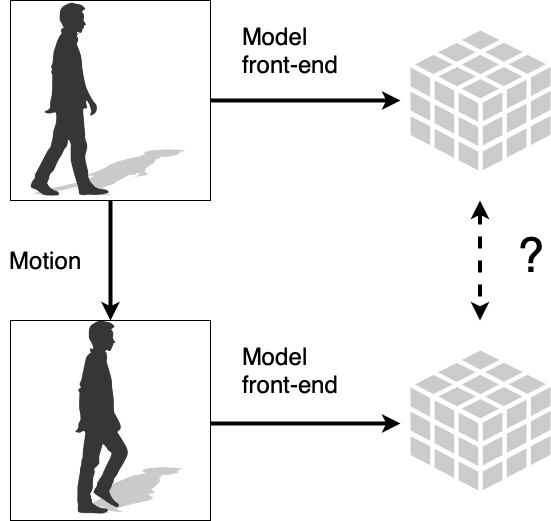
\includegraphics[width=0.6\linewidth]{img/video_latent_space_motion_analysis/motion_problem.png}
    \caption{The problem studied in this paper: if input images are related via motion, what is the relationship between the corresponding intermediate feature tensors?
    %Placeholder for "overview" image. Given a known geometric transformation between a pair of input images, and a feature tensor generated by partial deep model inference on the first image, how well can we estimate the corresponding feature tensor of the second image without using the deep model? \textcolor{red}{Since the focus in on motion in collaborative intelligence, I would suggest to change ``transformation'' to ``motion''}
    }
    \label{fig:video_latent_space_motion_analysis/overview}
\end{figure}

\textbf{Motion model.} Optical flow is a frequently used motion model in computer vision and video processing. In a ``2D+t'' model, $I(x,y,t)$ denotes pixel intensity at time $t$, at spatial position $(x,y)$. Under a constant-intensity assumption,  optical flow satisfies the following partial differential equation~\cite{Horn_Schunk_1981}:
% \vspace{-5pt}
\begin{equation}
    \frac{\partial I}{\partial x}v_x + \frac{\partial I}{\partial y}v_y + \frac{\partial I}{\partial t} = 0,
    \label{eq:video_latent_space_motion_analysis/2D+t_opt_flow}
\end{equation}
where $(v_x,v_y)$ represents the motion vector. For notational simplicity, in the analysis below we will use a ``1D+t'' model, which captures all the main ideas but keeps the equations shorter. In a ``1D+t'' model, $I(x,t)$ denotes intensity at position $x$ at time $t$, and the optical flow equation is
\begin{equation}
    \frac{\partial I}{\partial x}v  + \frac{\partial I}{\partial t} = 0,
    \label{eq:video_latent_space_motion_analysis/1D+t_opt_flow}
\end{equation}
with $v$ representing the motion.
%In typical deep models for computer vision applications, there are three basic operations applied to input images: convolutions, pointwise nonlinearities, and pooling operations.
We will analyze the effect of basic operations --- convolutions, pointwise nonlinearities, and pooling --- on \cref{eq:video_latent_space_motion_analysis/1D+t_opt_flow}, to gain insight into the relationship between input space motion and latent space motion.

\textbf{Convolution.} Let $f$ be a (spatial) filter kernel, then the optical flow after convolution is a solution to the following equation
% \vspace{-5pt}
\begin{equation}
    \frac{\partial}{\partial x}(f*I)v'  + \frac{\partial}{\partial t}(f*I) = 0,
    \label{eq:video_latent_space_motion_analysis/1D+t_conv}
\end{equation}
where $v'$ is the motion after the convolution. Since the convolution and differentiation are linear operations, we have
% \vspace{-3pt}
\begin{equation}
    f*\left(\frac{\partial I}{\partial x}v'  + \frac{\partial I}{\partial t} \right) = 0.
    \label{eq:video_latent_space_motion_analysis/1D+t_conv_2}
% \vspace{-2pt}
\end{equation}
Hence, solution $v$ from~\cref{eq:video_latent_space_motion_analysis/1D+t_opt_flow} is also a solution of~\cref{eq:video_latent_space_motion_analysis/1D+t_conv_2}, but~\cref{eq:video_latent_space_motion_analysis/1D+t_conv_2} could also have other solutions, besides those that satisfy~\cref{eq:video_latent_space_motion_analysis/1D+t_opt_flow}.

\textbf{Pointwise nonlinearity.} Nonlinear activations such as \texttt{sigmoid}, \texttt{ReLU}, etc., are commonly applied in a pointwise fashion on the output of convolutions in deep models. Let $\sigma(\cdot)$ denote such a pointwise nonlinearity, then the optical flow after this nonlinearity is a solution to the following equation
% \vspace{-3pt}
\begin{equation}
    \frac{\partial}{\partial x}\left[\sigma(I)\right]v'  + \frac{\partial}{\partial t}\left[\sigma(I)\right] = 0,
    \label{eq:video_latent_space_motion_analysis/1D+t_nonlin}
\end{equation}
where $v'$ is the motion after the pointwise nonlinearity. By using the chain rule of differentiation, the above equation can be rewritten as
% \vspace{-7pt}
\begin{equation}
    \sigma'(I)\cdot \left(\frac{\partial I}{\partial x}v'  + \frac{\partial I}{\partial t} \right) = 0.
    \label{eq:video_latent_space_motion_analysis/1D+t_nonlin_2}
\end{equation}
Hence, again, solution $v$ from~\cref{eq:video_latent_space_motion_analysis/1D+t_opt_flow} is also a solution of~\cref{eq:video_latent_space_motion_analysis/1D+t_nonlin_2}. It should be noted that~\cref{eq:video_latent_space_motion_analysis/1D+t_nonlin_2} may have solutions other than those from~\cref{eq:video_latent_space_motion_analysis/1D+t_opt_flow}. For example, in the region where inputs to \texttt{ReLU} are negative, the corresponding outputs will be zero, so $\sigma'(I)=0$. Hence, in those regions,~\cref{eq:video_latent_space_motion_analysis/1D+t_nonlin_2} will be satisfied for arbitrary $v'$. Nonetheless, the solution from~\cref{eq:video_latent_space_motion_analysis/1D+t_opt_flow} is still one of those arbitrary solutions.

\textbf{Pooling.} There are various forms of pooling, such as max-pooling, mean-pooling, learnt pooling (via strided convolutions), etc. All these can be decomposed into a sequence of two operations: a spatial operation (local maximum or convolution) followed by scale change (downsampling). Spatial convolution operations can be analyzed as above, and the conclusion is that motion before such an operation is also a solution to the optical flow equation after such an operation. Hence, we will focus here on the local maximum operation and the scale change.

\textit{Local maximum.} Consider the maximum of function $I(x,t)$ over a local spatial region $[x_0-h, x_0+h]$, at a given time $t$. We can approximate $I(x,t)$ as a locally-linear function, whose slope is the spatial derivative of $I$ at $x_0$, $\frac{\partial}{\partial x}I(x_0,t)$. If the derivative is positive, the maximum is $I(x_0+h,t)$, and if it is negative, it is $I(x_0-h,t)$. In the special case when the derivative is zero, any point in $[x_0-h, x_0+h]$, including the endpoints, is a maximum. From  Taylor series expansion of $I(x,t)$ around $x_0$ up to and including the first-order term,
% \vspace{-5pt}
\begin{equation}
    I(x_0 \pm \epsilon,t) \approx I(x_0,t) \pm \frac{\partial}{\partial x}I(x_0,t)\cdot \epsilon,
\end{equation}
for $|\epsilon| \leq h$. With such linear approximation, the local maximum of $I(x,t)$ over $[x_0-h, x_0+h]$ occurs either at $x_0+h$ or at $x_0-h$, depending on the sign of $\frac{\partial}{\partial x}I(x_0,t)$; if the derivative is zero, every point in the interval is a local maximum. Hence, the local maximum of $I(x,t)$ can be approximated as
% \vspace{-12pt}
\begin{equation}
\begin{split}
    &\max_{x\in[x_0-h, x_0+h]} I(x,t) \\
    & \qquad \approx I(x_0,t) + \sign\left(\frac{\partial}{\partial x}I(x_0,t)\right) \cdot \frac{\partial}{\partial x}I(x_0,t) \cdot h.
\end{split}
% \vspace{-6pt}
\label{eq:video_latent_space_motion_analysis/local_max}
\end{equation}
Let~\cref{eq:video_latent_space_motion_analysis/local_max} be the definition of $M(x_0,t)$, the function that takes on local spatial maximum values of $I(x,t)$ over windows of size $2h$. The optical flow after such a local maximum operation is described by
% \vspace{-3pt}
\begin{equation}
    \frac{\partial M}{\partial x}v'  + \frac{\partial M}{\partial t} = 0,
    \label{eq:video_latent_space_motion_analysis/1D+t_local_max}
\end{equation}
where $v'$ represents the motion after local spatial maximum operation. Using~\cref{eq:video_latent_space_motion_analysis/local_max} in~\cref{eq:video_latent_space_motion_analysis/1D+t_local_max}, after some manipulation we obtain the following equation
\begin{equation}
\begin{split}
    \frac{\partial I}{\partial x}v'  + \frac{\partial I}{\partial t} + \sign\left(\frac{\partial I}{\partial x}\right) \cdot \frac{\partial}{\partial x} \left( \frac{\partial I}{\partial x}v'  + \frac{\partial I}{\partial t}\right)\cdot h = 0.
\end{split}
\label{eq:video_latent_space_motion_analysis/1D+t_post_max}
\end{equation}
Note that if $v'$ satisfies the original optical flow equation~\cref{eq:video_latent_space_motion_analysis/1D+t_conv}, it will also satisfy~\cref{eq:video_latent_space_motion_analysis/1D+t_post_max}, hence pre-max motion $v$ is also one possible solution to post-max motion $v'$.

\textit{Scale change.} Finally, consider the change of spatial scale by a factor $s$, such that the new signal is $I'(x,t) =I(s\cdot x,t)$. The optical flow equation is now
\begin{equation}
    \frac{\partial I'}{\partial x}v'  + \frac{\partial I'}{\partial t} = 0.
    \label{eq:video_latent_space_motion_analysis/1D+t_scale_change}
\end{equation}
Since $\frac{\partial I'}{\partial x}=s\cdot \frac{\partial I}{\partial x}$ and $\frac{\partial I'}{\partial t}=\frac{\partial I}{\partial t}$, we conclude that $v'=v/s$, where $v$ is the solution to pre-scaling motion~\cref{eq:video_latent_space_motion_analysis/1D+t_opt_flow}. Hence, as expected, down-scaling the signal spatially by a factor of $2$ ($s=2$) would reduce the motion by a factor of $2$.

Combining the results of the above analyses, we conclude that convolutions, pointwise nonlinearities, and local maximum operations tend to be motion-preserving operations, in the sense that pre-operation motion is also a solution to post-operation optical flow, at least approximately. The operation with the most obvious impact on motion is scale change. Hence, when looking at latent-space motion at some layer in a deep model, we should expect to find motion similar to the input motion, but scaled down by a factor of $n^k$, where $k$ is the number of pooling operations (over $n\times n$ windows) between the input and the layer of interest. Specifically, if $\mathbf{v}$ is the motion vector at some position in the input frame, then at the corresponding spatial location in all the channels of the feature tensor we can expect to find the vector
\begin{equation}
    \mathbf{v}'\approx \mathbf{v}/n^k.
    \label{eq:video_latent_space_motion_analysis/mv_scale}
\end{equation}
In \cref{sec:video_latent_space_motion_analysis/experiments}, we will verify these conclusions experimentally.


\section{Experiments}
\label{sec:video_latent_space_motion_analysis/experiments}






% Implementation available at:
%
% https://gist.github.com/YodaEmbedding/c30f0d4045a945a5f92cdbfb9bddff3a
%
%
%NOTE: The title of the paper for the ICASSP version and arxiv versions is different. Is that intentional? \textcolor{red}{Yes, it is intentional, because this version contains more than the ICASSP version. Usually, we would keep the title if we had the same version posted on arXiv for open access. But if the papers are not exactly the same, as in this case, I think it is better to modify the title a bit, to avoid confusion.}
%\textcolor{green}{Since the arxiv paper is a subset of the other one, would it make sense to title it ``Latent Space Motion Analysis for Collaborative Intelligence (extended)''? It might also help ensure that any citations of the paper are concentrated and easier to identify against each other. This source,}
%\url{https://www.ncbi.nlm.nih.gov/pmc/articles/PMC5417409/#sec003title}
%\textcolor{green}{says ``Since preprints may extend beyond traditional published papers, [...],'' which suggests it is not uncommon to have extended preprints --- though, it doesn't provide any recommendations regarding titling. On a related note, papers on arxiv sometimes contain different versions, e.g. the BatchNorm paper has v1, v2, v3. In the last version, they've added a few paragraphs within the paper and within the conclusion that were not originally in v1.}

%\textcolor{blue}{%
An illustration of the correspondence between the input-space motion and latent-space motion was shown in \cref{fig:video_latent_space_motion_analysis/mv_overview}. This example was produced using a pair of frames from a video of a moving car.  The motion vectors were estimated using an exhaustive block-matching search at each pixel, which sought to minimize the sum of squared differences (SSD). In the input frames, whose resolution was $224 \times 224$, the block size of $31 \times 31$ around each pixel and
the search range of $\pm11$ were used. In the corresponding feature tensor channels, whose resolution was $28 \times 28$, the block size of $3 \times 3$ and a search range of $\pm5$ were used. Although the estimated motion vector fields are somewhat noisy, the similarity between the input-space motion and latent-space motion is evident.
%}

To examine the relationship between input-space and latent-space motion more closely, we performed several experiments with synthetic input-space motion. In this case, exact input-space motion is known, so relationship~\cref{eq:video_latent_space_motion_analysis/mv_scale} can be tested more reliably.  \cref{fig:video_latent_space_motion_analysis/examples} shows examples of various transformations (translation, rotation, stretching, shearing) applied to an input image of a dog. The second column displays several channels from the actual tensor produced by the transformed image, and the third column shows the corresponding channels produced by motion compensating the tensor of the original image via~\cref{eq:video_latent_space_motion_analysis/mv_scale}. The last column shows the difference between the actual and predicted tensor channels. Note that regions that cannot be predicted, such as regions ``entering the frame,'' were excluded from difference computation. As seen in \cref{fig:video_latent_space_motion_analysis/examples}, the model~\cref{eq:video_latent_space_motion_analysis/mv_scale} works reasonably well, and the differences between the actual and predicted tensors are low.


\begin{figure}[htbp]
    \centering
    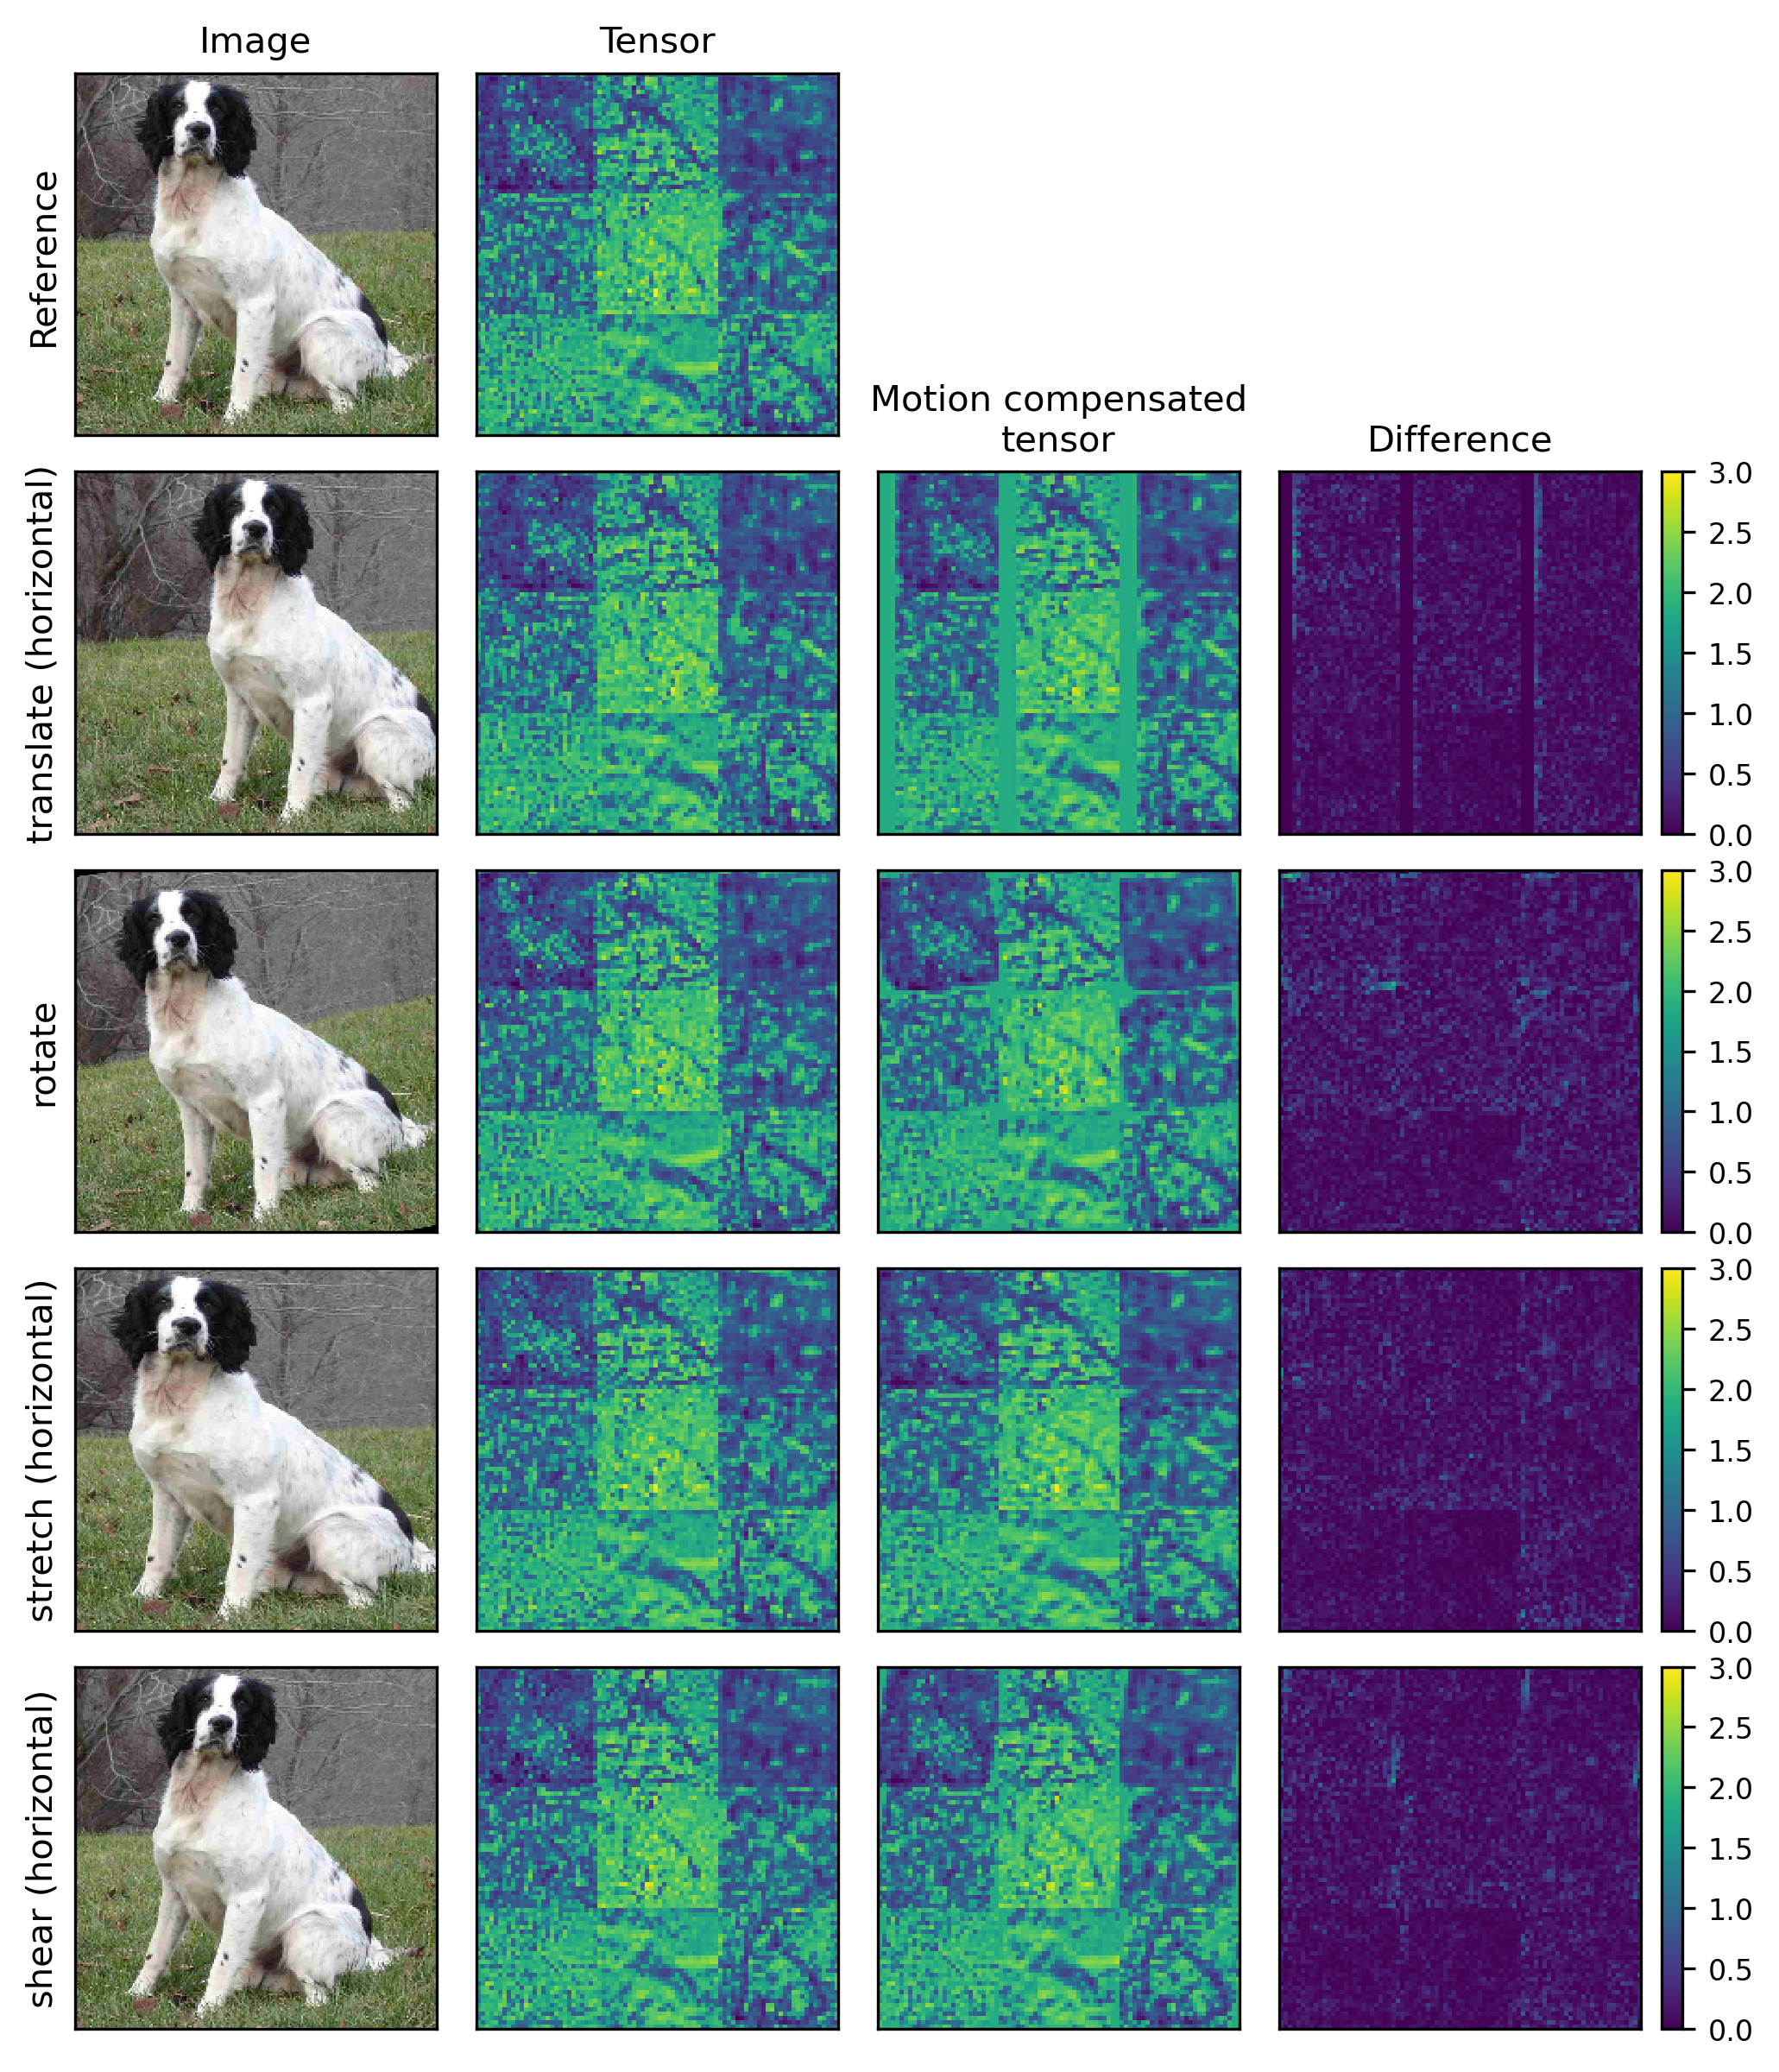
\includegraphics[width=0.95\linewidth]{img/video_latent_space_motion_analysis/examples.png}
    \caption{%
        Examples of motion transformations applied to reference image.
        The output tensors of ResNet-34's add\_3 layer are reliably predicted from only the reference tensor and known input-space motion. % within the pairs of input frames.
        %
        % COLUMNS
        % 1. frame
        % 2. contains "ground truth" tensors computed directly from frame
        % 3. contains predictions
        % 4. is (absolute) difference between third and second
        %
        % ROWS
        % 1. reference
        % 2. horizontal translate by 35 pixels
        % 3. rotate by 10 degrees
        % 4. horizontal scale by 1.2
        % 5. horizontal shear by 10 degrees
    }
    \label{fig:video_latent_space_motion_analysis/examples}
    % \vspace{-1.0\baselineskip}
\end{figure}


%Varied affine transformation parameters for ResNet-34 and DenseNet-121

%In the case of an affine transformation, ...



For quantitative evaluation, experiments were conducted on several layers of ResNet-34~\cite{ResNet} and DenseNet-121~\cite{DenseNet}. Normalized Root Mean Square Error (NRMSE)~\cite{wiki:NRMSE} was used for this purpose:
% \vspace{-7pt}
\begin{equation}
    \text{NRMSE} =  \frac{1}{R} \sqrt{\frac{1}{N} \sum_{i=1}^N (p_i - a_i)^2},
    \label{eq:video_latent_space_motion_analysis/NRMSE}
\end{equation}
where $a_i$ is the actual tensor value produced %by the front end of the DNN
from the transformed input, $p_i$
is the tensor value predicted using our motion model~\cref{eq:video_latent_space_motion_analysis/mv_scale}, $N$ is the number of elements in the feature tensor, and $R$ is the dynamic range. Again, regions that cannot be predicted were excluded from NRMSE computation. \cref{fig:video_latent_space_motion_analysis/transform} shows NRMSE computed across a range of parameters for several transformations, at various layers of the two DNNs. %The brackets in the legends indicate the layer index in the DNN, for example (4/37) means 4$^\text{th}$ out of 37 layers.


\begin{figure*}[tb]
    \centering
    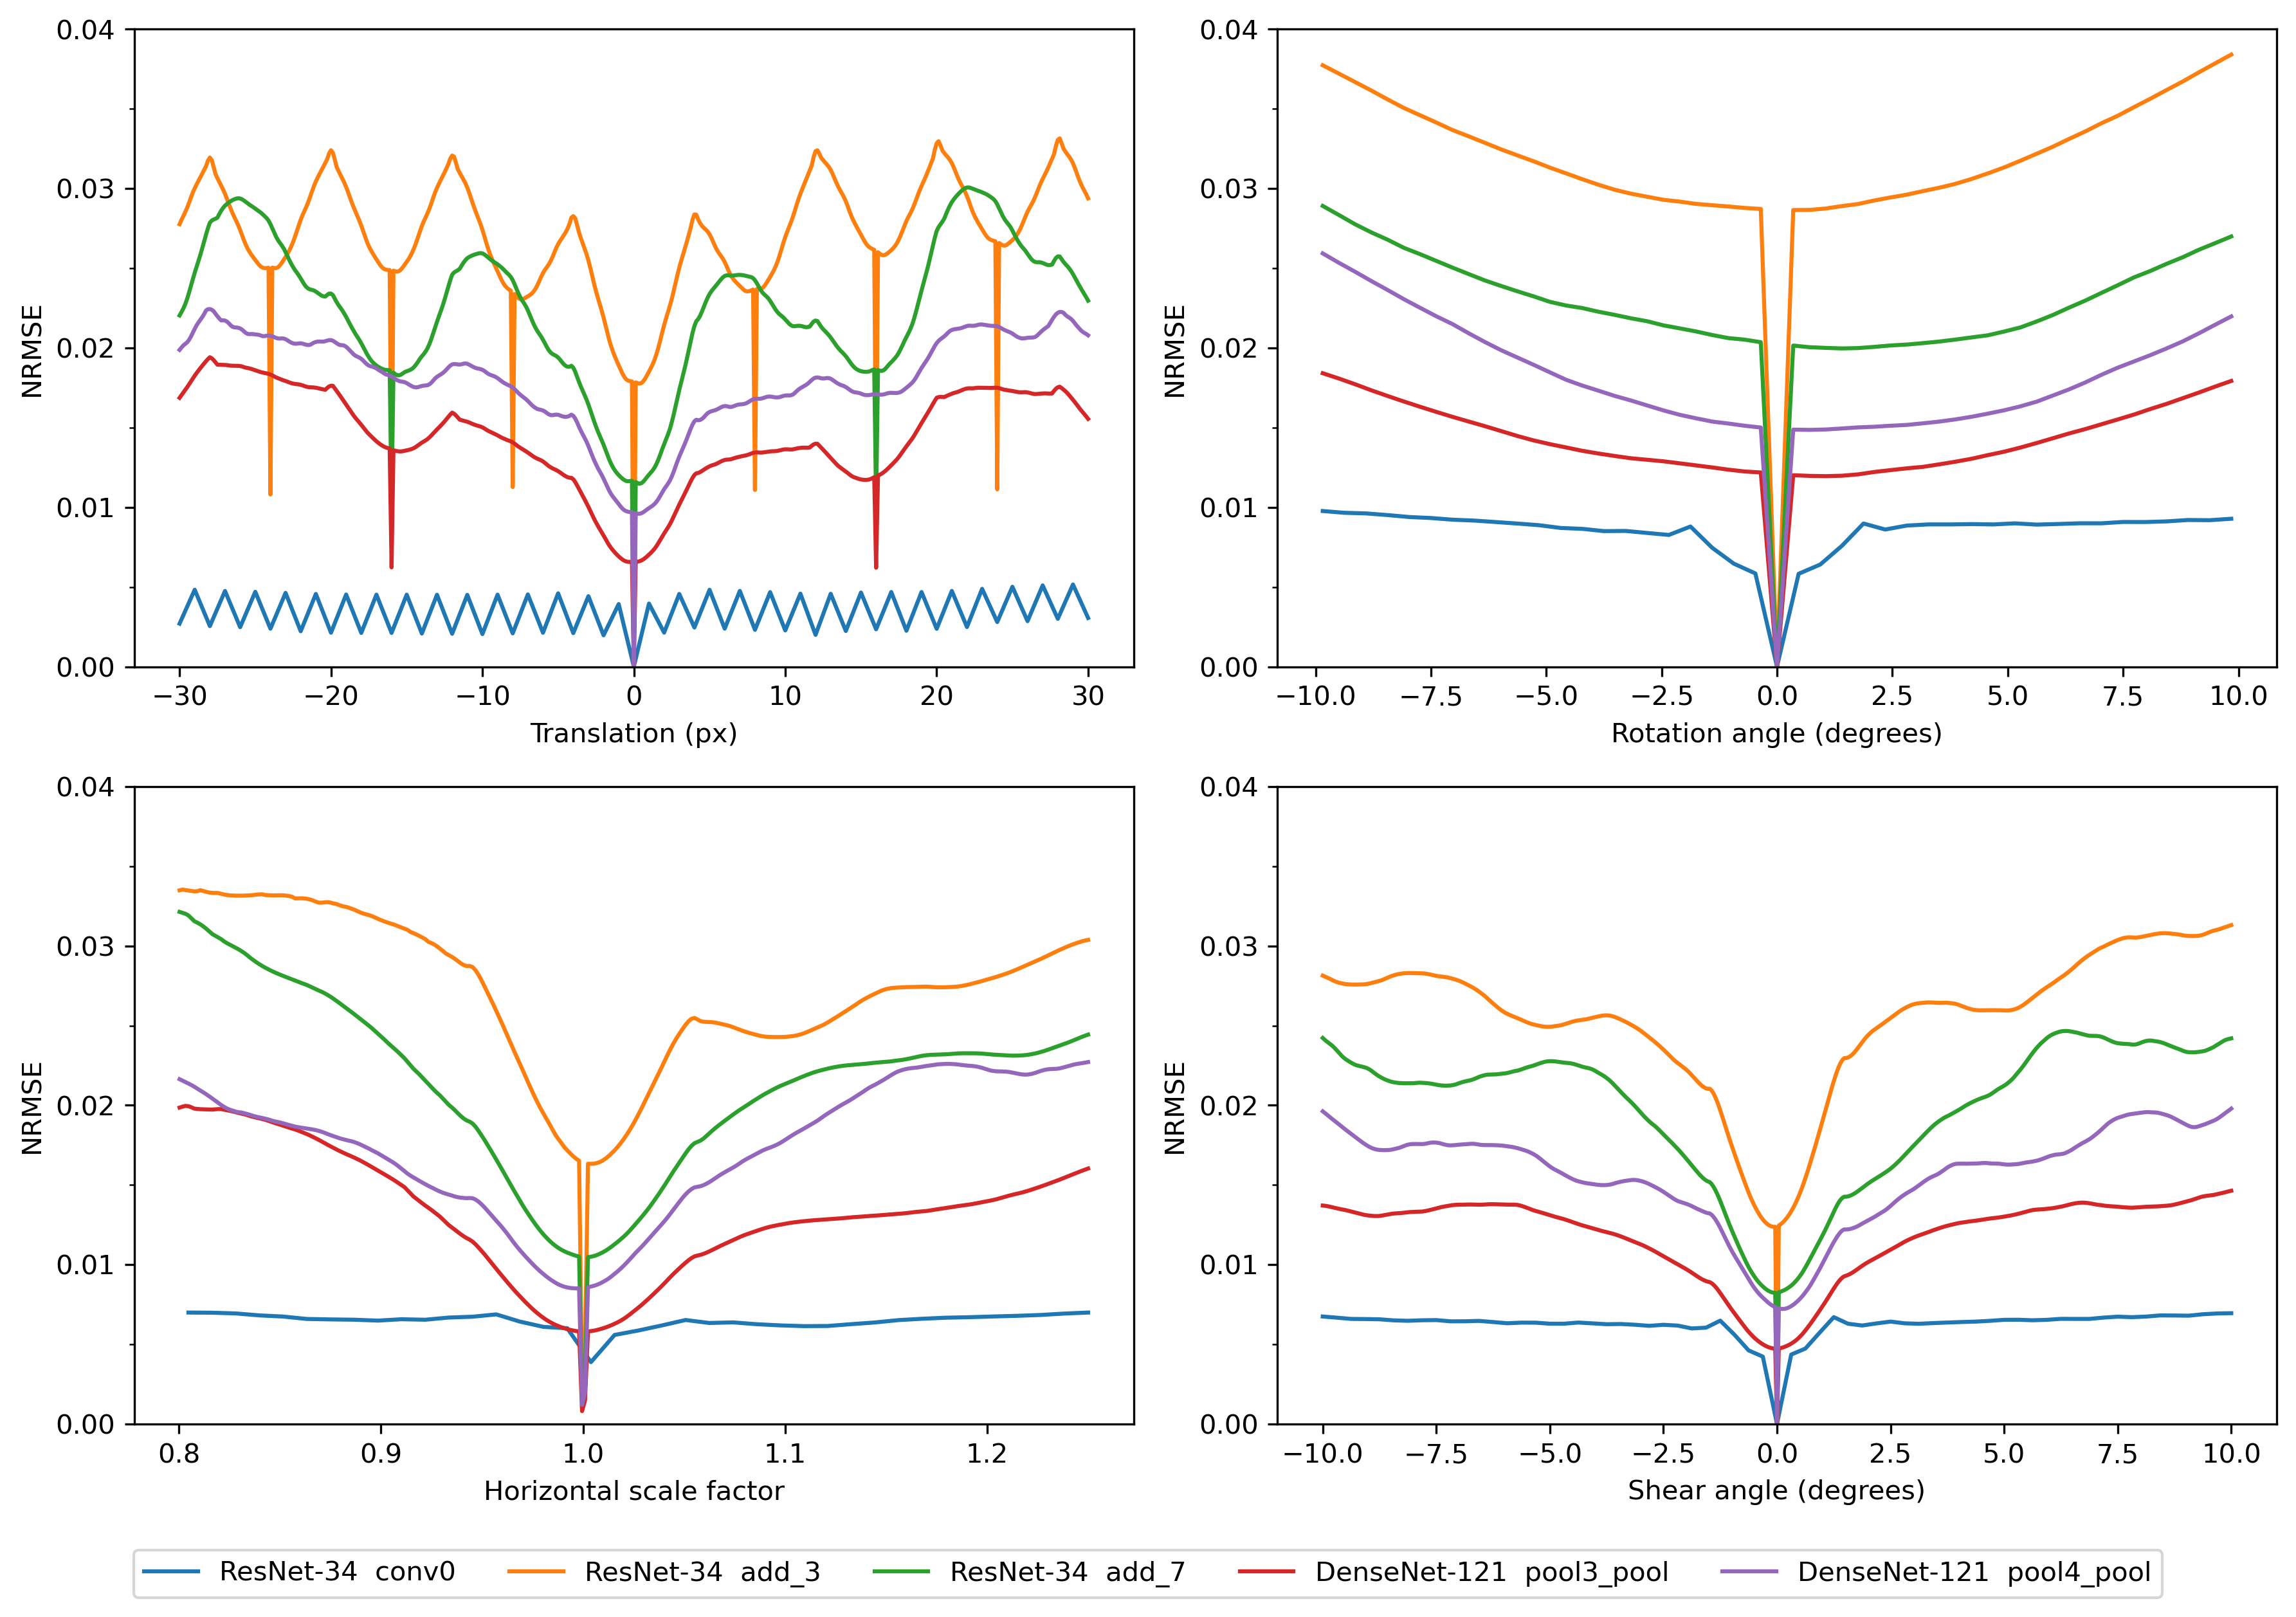
\includegraphics[width=\linewidth]{img/video_latent_space_motion_analysis/nrmse/transform_curves-all.png}
    \caption{%
        NRMSE across parameter ranges for translation (top-left), rotation (top-right), scaling (bottom-left), and shear (bottom-right).
        For translation, NRMSE local minima occur when the input-space shifts correspond to integer latent-space shifts in~\cref{eq:video_latent_space_motion_analysis/mv_scale}.%
    }
    \label{fig:video_latent_space_motion_analysis/transform}
%    \vspace{-10pt}
\end{figure*}



%$R$ is computed from dynamic range of tensor

%after masking out the "non-transformable regions"




%Determine threshold value for what a "typical" codec would see for NRMSE block based matching in typical situation




%The other curves have different periods for translation

As seen in \cref{fig:video_latent_space_motion_analysis/transform}, NRMSE goes up to about 0.04 for reasonable ranges of transformation parameters. How good is this? To answer this question, we set out to find the typical values of NRMSE found in conventional motion-compensated frame prediction.
In a recent study~\cite{Choi_TCSVT_2020}, the quality of frames predicted by conventional motion estimation and motion compensation (MEMC) in High Efficiency Video Coding (HEVC)~\cite{H.265} was compared against a DNN developed for frame prediction. From Table~III in~\cite{Choi_TCSVT_2020}, the luminance Peak Signal to Noise Ratio (PSNR) of frames predicted uni-directionally by the DNN and conventional HEVC MEMC was in the range 27--41 dB over several HEVC test sequences. NRMSE can be computed from PSNR as
% \vspace{-2pt}
\begin{equation}
    \text{NRMSE} = \frac{1}{256}\sqrt{\frac{255^2}{10^{\text{PSNR}/10}}},
% \vspace{-2pt}
\end{equation}
so the PSNR range of 27--41 dB corresponds to the NRMSE range of 0.009--0.044. These levels of NRMSE are indicative of how much motion models used in video coding deviate from the true motion. As seen in \cref{fig:video_latent_space_motion_analysis/transform}, the model~\cref{eq:video_latent_space_motion_analysis/mv_scale} produces NRMSE in the same range, so the accuracy of~\cref{eq:video_latent_space_motion_analysis/mv_scale} is comparable to the accuracy of common motion models used in video coding. Another illustration of this is presented in \cref{fig:video_latent_space_motion_analysis/mse/histogram}, which shows the histogram of NRMSE computed across a range of affine transformation parameters.  Hence,~\cref{eq:video_latent_space_motion_analysis/mv_scale} represents a good starting point for development of latent-space motion compensation.

\begin{figure}[htbp]
    \centering
    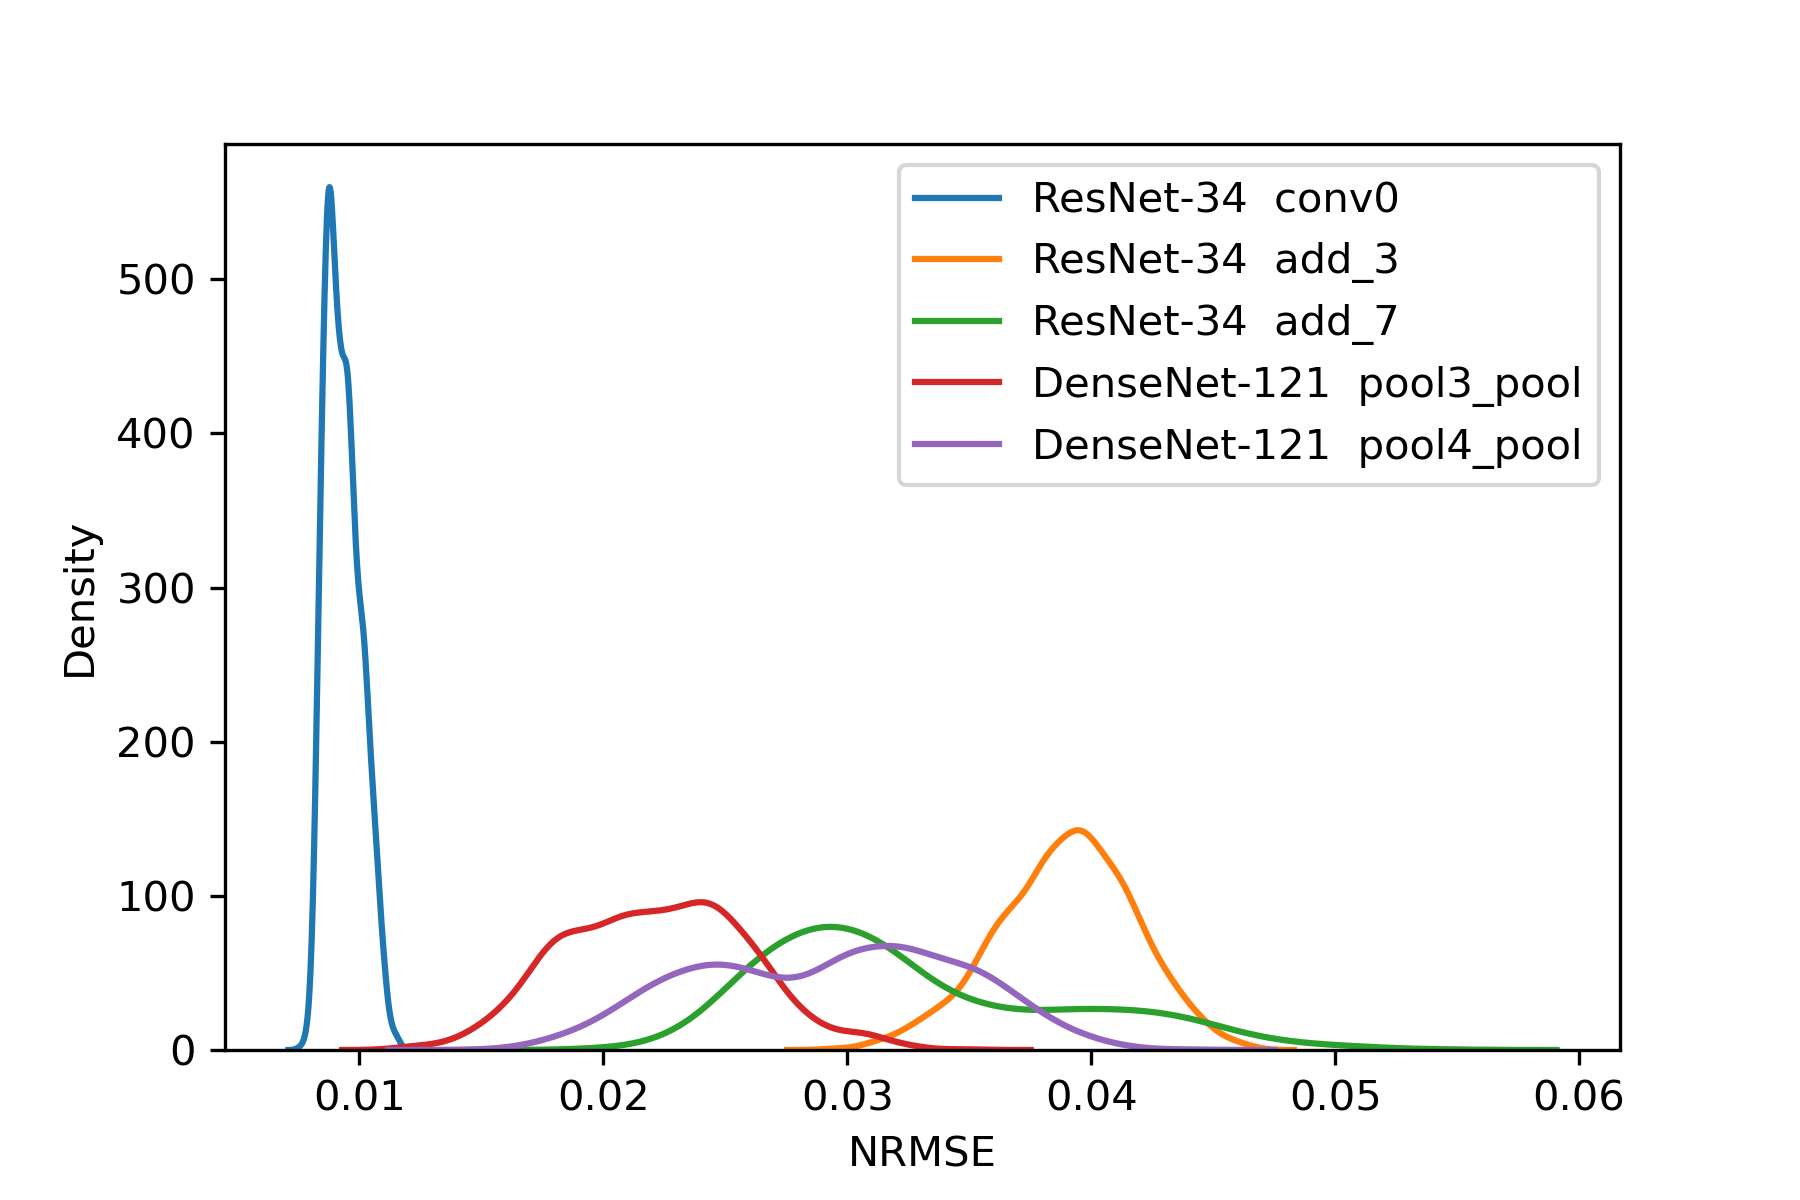
\includegraphics[width=\linewidth]{img/video_latent_space_motion_analysis/nrmse/random.png}
    \caption{%
        NRMSE histogram computed for an affine motion model~\cite{wang_etal_2002} over the combination of the following seven independent uniformly distributed parameters: x- and y-translation ($\pm 32$ px), x- and y-scaling (0.95--1.05), x- and y-shearing ($\pm 5^{\circ}$), and rotation ($\pm 10^{\circ}$).%
        %These roughly model the motion between successive frames in a video sequence.%
    }
    \label{fig:video_latent_space_motion_analysis/mse/histogram}
\end{figure}




\section{Conclusions}
\label{sec:video_latent_space_motion_analysis/conclusions}
Using the concept of optical flow, in this paper we analyzed motion in the latent space of a deep model induced by the motion in the input space, and showed that motion tends to be approximately preserved in the channels of intermediate feature tensors. These findings suggest that motion estimation, compensation, and analysis methods developed for conventional video signals should be able to provide a good starting point for latent-space motion processing, such as motion-compensated prediction and compression, tracking, action recognition, and other applications.
%Another intriguing prospect, which requires further analysis, is the possibility of inferring input-space motion from latent-space features.


\chapter{Latent space motion analysis for collaborative intelligence}
% \chapter{Latent Space Motion Analysis for Collaborative Intelligence}
\label{ch:video_latent_space_motion_analysis}

% Changes made:
%
% Replacements:
% :%s/eq:/eq:video_latent_space_motion_analysis\//g
% :%s/fig:/fig:video_latent_space_motion_analysis\//g
% :%s/sec:/sec:video_latent_space_motion_analysis\//g
% :%s/img\//img\/video_latent_space_motion_analysis\//g
% :%s/Duan2020VideoCF/duan2020vcm/g
% :%s/Choi2018NearLosslessDF/choi2018mmsp/g
%
% Removals:
% \vspace{...}
% \FloatBarrier
%
% Reorder:
% figures




% \usepackage{flushend}
% \usepackage{fancyhdr}
% \pagestyle{fancy}
% \fancyhf{}
% \renewcommand{\headrulewidth}{0pt}% Header rule
% \renewcommand{\footrulewidth}{0pt}% Footer rule
% \fancyhead[C]{}
%
% \fancypagestyle{firstpage}{% Page style for first page
%   \fancyhf{}% Clear header/footer
%   \renewcommand{\headrulewidth}{0pt}% Header rule
%   \renewcommand{\footrulewidth}{0pt}% Footer rule
%   \fancyhead[C]{\vspace{-2.2cm}Extended version of the paper ``Latent Space Motion Analysis for Collaborative Intelligence,'' to be presented at the IEEE International Conference on Acoustics, Speech and Signal Processing (ICASSP), Toronto, Canada, June 6-1, 2021. \vspace{0.3cm}}
% }




\begin{center}
  \small
  Notice: This chapter has been reproduced from the paper~\cite{ulhaq2021analysis}.
\end{center}




\begin{chapabstract}
When the input to a deep neural network (DNN) is a video signal, a sequence of feature tensors is produced at the intermediate layers of the model. If neighboring frames of the input video are related through motion, a natural question is, ``what is the relationship between the corresponding feature tensors?'' By analyzing the effect of common DNN operations on optical flow, we show that the motion present in each channel of a feature tensor is approximately equal to the scaled version of the input motion. The analysis is validated through experiments utilizing common motion models. %These results will be useful in collaborative intelligence applications where sequences of feature tensors need to be compressed or further analyzed.
\end{chapabstract}


% \begin{keywords}
% Collaborative intelligence, latent space motion, feature domain motion, feature compression
% \end{keywords}




\section{Introduction}

Collaborative intelligence (CI)~\cite{Bajic_etal_ICASSP21} has emerged as a promising strategy to bring AI ``to the edge.'' In a typical CI system (\cref{fig:video_latent_space_motion_analysis/CI_system}), a deep neural network (DNN) is split into two parts: the edge sub-model, deployed on the edge device near the sensor, and the cloud sub-model deployed in the cloud. Intermediate features produced by the edge sub-model are transferred from the edge device to the cloud. It has been shown that such a strategy may provide better energy efficiency~\cite{kang2017neurosurgeon,jointdnn}, lower latency~\cite{kang2017neurosurgeon,jointdnn,ulhaq2019neurips_demo}, and lower bitrates over the communication channel~\cite{dfc_for_collab_object_detection,choi2018mmsp}, compared to more traditional cloud-based analytics where the input signal is directly sent to the cloud. These potential benefits will find a number of applications in areas such as intelligent sensing~\cite{Chen19} and video coding for machines~\cite{MPEG_VCM_CFE,duan2020vcm}. In particular, compression of intermediate features has become an important research problem, with a number of recent developments~\cite{Saeed_ICIP19,Hyomin_ICASSP20,Saeed_ICASSP20,Bob_ICME20, Saeed2020pareto_arxiv} for the case when the input to the edge sub-model is a still image.

When the input to the edge sub-model is video, its output is a sequence of feature tensors produced from successive frames in the input video. This sequence of feature tensors needs to be compressed prior to transmission and then decoded in the cloud for further processing. Since motion plays such an important role in video processing and compression, we are motivated to examine whether any similar relationship exists in the latent space among the feature tensors. Our theoretical and experimental results show that, indeed, motion from the input video is approximately preserved in the channels of the feature tensor. %\textcolor{blue}{
An illustration of this is presented in \cref{fig:video_latent_space_motion_analysis/mv_overview}, where the estimated input-space motion field is shown on the left, and the estimated motion fields in several feature tensor channels are shown on the right.
%}
These findings suggest that methods for motion estimation, compensation, and analysis that have been developed for conventional video processing and compression may provide a solid starting point for equivalent operations in the latent space.

\begin{figure}[htbp]
    \centering
    \vspace{\baselineskip}%
    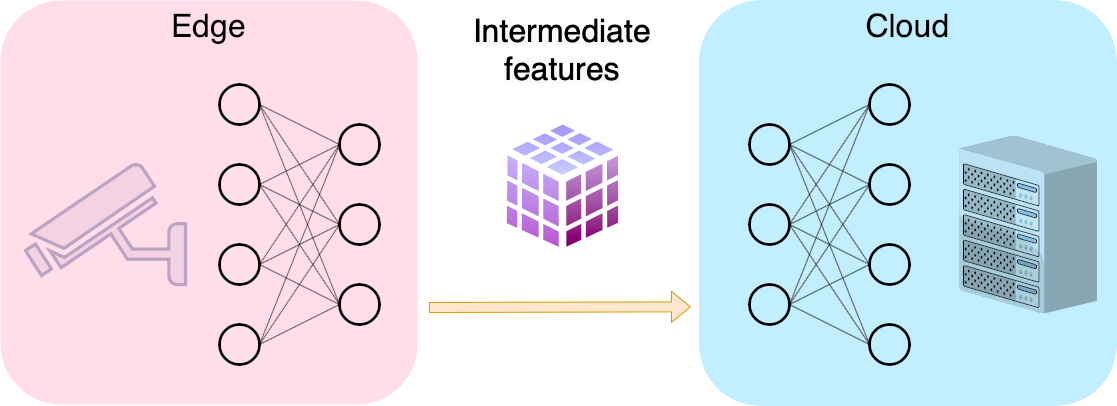
\includegraphics[width=\columnwidth]{img/video_latent_space_motion_analysis/CI_system.png}%
    \vspace{0.5\baselineskip}%
    \caption{Basic collaborative intelligence system.}
    \label{fig:video_latent_space_motion_analysis/CI_system}
    % \vspace{-1.0\baselineskip}
\end{figure}

\begin{figure}[htbp]
    \centering
    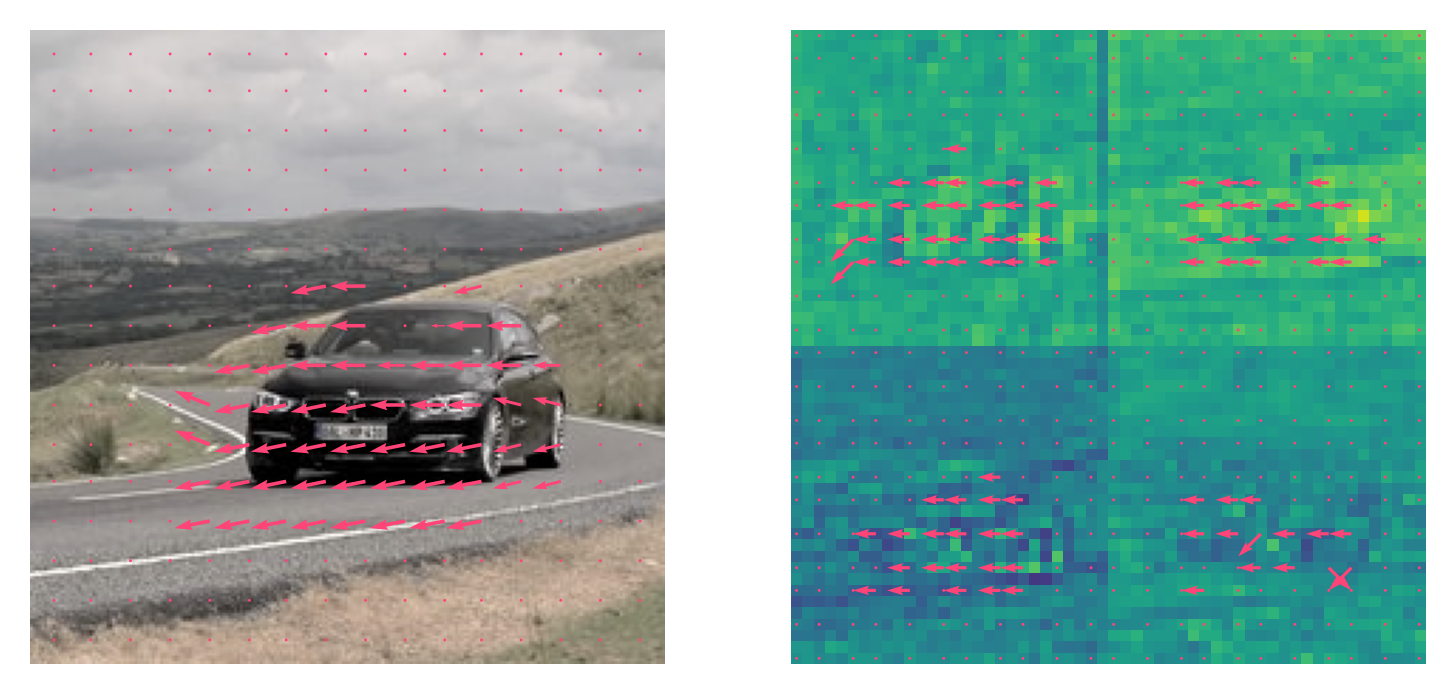
\includegraphics[width=\columnwidth]{img/video_latent_space_motion_analysis/mv_car.png}
    \caption{%
        Motion estimates for input frames (left) and
        select channels from the output of ResNet-34's add\_3 layer (right).
    }
    \label{fig:video_latent_space_motion_analysis/mv_overview}
    % \vspace{-1.0\baselineskip}
\end{figure}

The paper is organized as follows. In \cref{sec:video_latent_space_motion_analysis/motion_analysis}, we analyze the actions of typical operations found in deep convolutional neural networks on optical flow in the input signal, and show that these operations tend to preserve the optical flow, at least approximately, with an appropriate scale. In \cref{sec:video_latent_space_motion_analysis/experiments} we provide empirical support for the theoretical analysis from \cref{sec:video_latent_space_motion_analysis/motion_analysis}. %using canonical motions such as translation, rotation, and scale change.
Finally, \cref{sec:video_latent_space_motion_analysis/conclusions} concludes the paper.


% \FloatBarrier


%The problem may be formulated as follows: Let $x$ be an input frame and $y = f(x)$ be its corresponding output at an intermediate layer within the deep model. Let $x'$ be another input frame that may be related to $x$ by a transformation $x' \approx g(x)$. Provided only $y$ and $g$, can we reliably predict the output $y' = f(x')$?

%For simplicity, assume that the intermediate layer operation is a 2x2 max pool of stride 2. Then in the case of simple translation of the contents of the input frame by $(u, v)$, we may state:

%\[x'_{i, j} = (g_{u, v}(x))_{i, j} = x_{i - u, j - v}\]

%\[y'_{i, j} = y_{i - \sfrac{u}{2}, j - \sfrac{v}{2}}\]

%More generally, for an affine transformation $A(M, u, v)$ (comprised of a linear transformation $M$ and translation $(u, v)$), we may state:

% TODO simplify notation

%\[x'_{i, j} = (g_{u, v}(x))_{i, j} = x_{A^{-1}(M, u, v)(i, j)}\]

%\[y'_{i, j} = y_{A^{-1}(M, \sfrac{u}{2}, \sfrac{v}{2})(i, j)}\]





\section{Latent space motion analysis}
\label{sec:video_latent_space_motion_analysis/motion_analysis}

The basic problem studied in this paper is illustrated in \cref{fig:video_latent_space_motion_analysis/overview}. Consider two images (video frames) input to the edge sub-model of a CI system. It is common to represent their relationship via a motion model. The question we seek to answer here is, ``what is the relationship between the corresponding feature tensors produced by the edge sub-model?'' To answer this question, we will look at the processing pipeline between the input image and a given channel of a feature tensor. In most deep models for computer vision applications, this processing pipeline consists of a sequence of basic operations: convolutions, pointwise nonlinearities, and pooling.  We will show that each of these operations tends to preserve motion, at least approximately, in a certain sense, and from this we will conclude that (approximate) input motion may be observed in individual channels of a feature tensor.

\begin{figure}[htbp]
    \centering
    %\includegraphics[width=0.7\linewidth]{img/video_latent_space_motion_analysis/overview.png}
    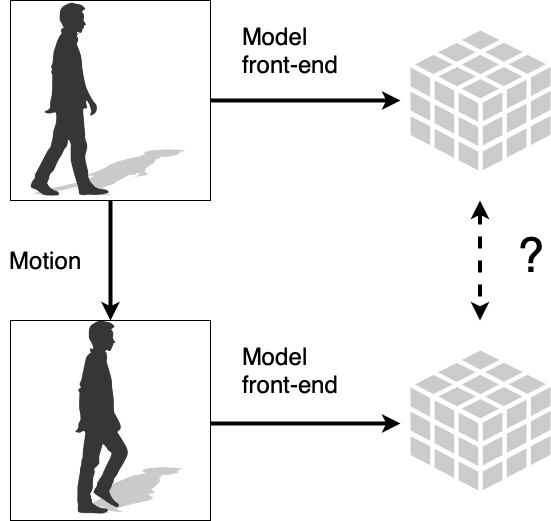
\includegraphics[width=0.6\linewidth]{img/video_latent_space_motion_analysis/motion_problem.png}
    \caption{The problem studied in this paper: if input images are related via motion, what is the relationship between the corresponding intermediate feature tensors?
    %Placeholder for "overview" image. Given a known geometric transformation between a pair of input images, and a feature tensor generated by partial deep model inference on the first image, how well can we estimate the corresponding feature tensor of the second image without using the deep model? \textcolor{red}{Since the focus in on motion in collaborative intelligence, I would suggest to change ``transformation'' to ``motion''}
    }
    \label{fig:video_latent_space_motion_analysis/overview}
\end{figure}

\textbf{Motion model.} Optical flow is a frequently used motion model in computer vision and video processing. In a ``2D+t'' model, $I(x,y,t)$ denotes pixel intensity at time $t$, at spatial position $(x,y)$. Under a constant-intensity assumption,  optical flow satisfies the following partial differential equation~\cite{Horn_Schunk_1981}:
% \vspace{-5pt}
\begin{equation}
    \frac{\partial I}{\partial x}v_x + \frac{\partial I}{\partial y}v_y + \frac{\partial I}{\partial t} = 0,
    \label{eq:video_latent_space_motion_analysis/2D+t_opt_flow}
\end{equation}
where $(v_x,v_y)$ represents the motion vector. For notational simplicity, in the analysis below we will use a ``1D+t'' model, which captures all the main ideas but keeps the equations shorter. In a ``1D+t'' model, $I(x,t)$ denotes intensity at position $x$ at time $t$, and the optical flow equation is
\begin{equation}
    \frac{\partial I}{\partial x}v  + \frac{\partial I}{\partial t} = 0,
    \label{eq:video_latent_space_motion_analysis/1D+t_opt_flow}
\end{equation}
with $v$ representing the motion.
%In typical deep models for computer vision applications, there are three basic operations applied to input images: convolutions, pointwise nonlinearities, and pooling operations.
We will analyze the effect of basic operations --- convolutions, pointwise nonlinearities, and pooling --- on \cref{eq:video_latent_space_motion_analysis/1D+t_opt_flow}, to gain insight into the relationship between input space motion and latent space motion.

\textbf{Convolution.} Let $f$ be a (spatial) filter kernel, then the optical flow after convolution is a solution to the following equation
% \vspace{-5pt}
\begin{equation}
    \frac{\partial}{\partial x}(f*I)v'  + \frac{\partial}{\partial t}(f*I) = 0,
    \label{eq:video_latent_space_motion_analysis/1D+t_conv}
\end{equation}
where $v'$ is the motion after the convolution. Since the convolution and differentiation are linear operations, we have
% \vspace{-3pt}
\begin{equation}
    f*\left(\frac{\partial I}{\partial x}v'  + \frac{\partial I}{\partial t} \right) = 0.
    \label{eq:video_latent_space_motion_analysis/1D+t_conv_2}
% \vspace{-2pt}
\end{equation}
Hence, solution $v$ from~\cref{eq:video_latent_space_motion_analysis/1D+t_opt_flow} is also a solution of~\cref{eq:video_latent_space_motion_analysis/1D+t_conv_2}, but~\cref{eq:video_latent_space_motion_analysis/1D+t_conv_2} could also have other solutions, besides those that satisfy~\cref{eq:video_latent_space_motion_analysis/1D+t_opt_flow}.

\textbf{Pointwise nonlinearity.} Nonlinear activations such as \texttt{sigmoid}, \texttt{ReLU}, etc., are commonly applied in a pointwise fashion on the output of convolutions in deep models. Let $\sigma(\cdot)$ denote such a pointwise nonlinearity, then the optical flow after this nonlinearity is a solution to the following equation
% \vspace{-3pt}
\begin{equation}
    \frac{\partial}{\partial x}\left[\sigma(I)\right]v'  + \frac{\partial}{\partial t}\left[\sigma(I)\right] = 0,
    \label{eq:video_latent_space_motion_analysis/1D+t_nonlin}
\end{equation}
where $v'$ is the motion after the pointwise nonlinearity. By using the chain rule of differentiation, the above equation can be rewritten as
% \vspace{-7pt}
\begin{equation}
    \sigma'(I)\cdot \left(\frac{\partial I}{\partial x}v'  + \frac{\partial I}{\partial t} \right) = 0.
    \label{eq:video_latent_space_motion_analysis/1D+t_nonlin_2}
\end{equation}
Hence, again, solution $v$ from~\cref{eq:video_latent_space_motion_analysis/1D+t_opt_flow} is also a solution of~\cref{eq:video_latent_space_motion_analysis/1D+t_nonlin_2}. It should be noted that~\cref{eq:video_latent_space_motion_analysis/1D+t_nonlin_2} may have solutions other than those from~\cref{eq:video_latent_space_motion_analysis/1D+t_opt_flow}. For example, in the region where inputs to \texttt{ReLU} are negative, the corresponding outputs will be zero, so $\sigma'(I)=0$. Hence, in those regions,~\cref{eq:video_latent_space_motion_analysis/1D+t_nonlin_2} will be satisfied for arbitrary $v'$. Nonetheless, the solution from~\cref{eq:video_latent_space_motion_analysis/1D+t_opt_flow} is still one of those arbitrary solutions.

\textbf{Pooling.} There are various forms of pooling, such as max-pooling, mean-pooling, learnt pooling (via strided convolutions), etc. All these can be decomposed into a sequence of two operations: a spatial operation (local maximum or convolution) followed by scale change (downsampling). Spatial convolution operations can be analyzed as above, and the conclusion is that motion before such an operation is also a solution to the optical flow equation after such an operation. Hence, we will focus here on the local maximum operation and the scale change.

\textit{Local maximum.} Consider the maximum of function $I(x,t)$ over a local spatial region $[x_0-h, x_0+h]$, at a given time $t$. We can approximate $I(x,t)$ as a locally-linear function, whose slope is the spatial derivative of $I$ at $x_0$, $\frac{\partial}{\partial x}I(x_0,t)$. If the derivative is positive, the maximum is $I(x_0+h,t)$, and if it is negative, it is $I(x_0-h,t)$. In the special case when the derivative is zero, any point in $[x_0-h, x_0+h]$, including the endpoints, is a maximum. From  Taylor series expansion of $I(x,t)$ around $x_0$ up to and including the first-order term,
% \vspace{-5pt}
\begin{equation}
    I(x_0 \pm \epsilon,t) \approx I(x_0,t) \pm \frac{\partial}{\partial x}I(x_0,t)\cdot \epsilon,
\end{equation}
for $|\epsilon| \leq h$. With such linear approximation, the local maximum of $I(x,t)$ over $[x_0-h, x_0+h]$ occurs either at $x_0+h$ or at $x_0-h$, depending on the sign of $\frac{\partial}{\partial x}I(x_0,t)$; if the derivative is zero, every point in the interval is a local maximum. Hence, the local maximum of $I(x,t)$ can be approximated as
% \vspace{-12pt}
\begin{equation}
\begin{split}
    &\max_{x\in[x_0-h, x_0+h]} I(x,t) \\
    & \qquad \approx I(x_0,t) + \sign\left(\frac{\partial}{\partial x}I(x_0,t)\right) \cdot \frac{\partial}{\partial x}I(x_0,t) \cdot h.
\end{split}
% \vspace{-6pt}
\label{eq:video_latent_space_motion_analysis/local_max}
\end{equation}
Let~\cref{eq:video_latent_space_motion_analysis/local_max} be the definition of $M(x_0,t)$, the function that takes on local spatial maximum values of $I(x,t)$ over windows of size $2h$. The optical flow after such a local maximum operation is described by
% \vspace{-3pt}
\begin{equation}
    \frac{\partial M}{\partial x}v'  + \frac{\partial M}{\partial t} = 0,
    \label{eq:video_latent_space_motion_analysis/1D+t_local_max}
\end{equation}
where $v'$ represents the motion after local spatial maximum operation. Using~\cref{eq:video_latent_space_motion_analysis/local_max} in~\cref{eq:video_latent_space_motion_analysis/1D+t_local_max}, after some manipulation we obtain the following equation
\begin{equation}
\begin{split}
    \frac{\partial I}{\partial x}v'  + \frac{\partial I}{\partial t} + \sign\left(\frac{\partial I}{\partial x}\right) \cdot \frac{\partial}{\partial x} \left( \frac{\partial I}{\partial x}v'  + \frac{\partial I}{\partial t}\right)\cdot h = 0.
\end{split}
\label{eq:video_latent_space_motion_analysis/1D+t_post_max}
\end{equation}
Note that if $v'$ satisfies the original optical flow equation~\cref{eq:video_latent_space_motion_analysis/1D+t_conv}, it will also satisfy~\cref{eq:video_latent_space_motion_analysis/1D+t_post_max}, hence pre-max motion $v$ is also one possible solution to post-max motion $v'$.

\textit{Scale change.} Finally, consider the change of spatial scale by a factor $s$, such that the new signal is $I'(x,t) =I(s\cdot x,t)$. The optical flow equation is now
\begin{equation}
    \frac{\partial I'}{\partial x}v'  + \frac{\partial I'}{\partial t} = 0.
    \label{eq:video_latent_space_motion_analysis/1D+t_scale_change}
\end{equation}
Since $\frac{\partial I'}{\partial x}=s\cdot \frac{\partial I}{\partial x}$ and $\frac{\partial I'}{\partial t}=\frac{\partial I}{\partial t}$, we conclude that $v'=v/s$, where $v$ is the solution to pre-scaling motion~\cref{eq:video_latent_space_motion_analysis/1D+t_opt_flow}. Hence, as expected, down-scaling the signal spatially by a factor of $2$ ($s=2$) would reduce the motion by a factor of $2$.

Combining the results of the above analyses, we conclude that convolutions, pointwise nonlinearities, and local maximum operations tend to be motion-preserving operations, in the sense that pre-operation motion is also a solution to post-operation optical flow, at least approximately. The operation with the most obvious impact on motion is scale change. Hence, when looking at latent-space motion at some layer in a deep model, we should expect to find motion similar to the input motion, but scaled down by a factor of $n^k$, where $k$ is the number of pooling operations (over $n\times n$ windows) between the input and the layer of interest. Specifically, if $\mathbf{v}$ is the motion vector at some position in the input frame, then at the corresponding spatial location in all the channels of the feature tensor we can expect to find the vector
\begin{equation}
    \mathbf{v}'\approx \mathbf{v}/n^k.
    \label{eq:video_latent_space_motion_analysis/mv_scale}
\end{equation}
In \cref{sec:video_latent_space_motion_analysis/experiments}, we will verify these conclusions experimentally.


\section{Experiments}
\label{sec:video_latent_space_motion_analysis/experiments}






% Implementation available at:
%
% https://gist.github.com/YodaEmbedding/c30f0d4045a945a5f92cdbfb9bddff3a
%
%
%NOTE: The title of the paper for the ICASSP version and arxiv versions is different. Is that intentional? \textcolor{red}{Yes, it is intentional, because this version contains more than the ICASSP version. Usually, we would keep the title if we had the same version posted on arXiv for open access. But if the papers are not exactly the same, as in this case, I think it is better to modify the title a bit, to avoid confusion.}
%\textcolor{green}{Since the arxiv paper is a subset of the other one, would it make sense to title it ``Latent Space Motion Analysis for Collaborative Intelligence (extended)''? It might also help ensure that any citations of the paper are concentrated and easier to identify against each other. This source,}
%\url{https://www.ncbi.nlm.nih.gov/pmc/articles/PMC5417409/#sec003title}
%\textcolor{green}{says ``Since preprints may extend beyond traditional published papers, [...],'' which suggests it is not uncommon to have extended preprints --- though, it doesn't provide any recommendations regarding titling. On a related note, papers on arxiv sometimes contain different versions, e.g. the BatchNorm paper has v1, v2, v3. In the last version, they've added a few paragraphs within the paper and within the conclusion that were not originally in v1.}

%\textcolor{blue}{%
An illustration of the correspondence between the input-space motion and latent-space motion was shown in \cref{fig:video_latent_space_motion_analysis/mv_overview}. This example was produced using a pair of frames from a video of a moving car.  The motion vectors were estimated using an exhaustive block-matching search at each pixel, which sought to minimize the sum of squared differences (SSD). In the input frames, whose resolution was $224 \times 224$, the block size of $31 \times 31$ around each pixel and
the search range of $\pm11$ were used. In the corresponding feature tensor channels, whose resolution was $28 \times 28$, the block size of $3 \times 3$ and a search range of $\pm5$ were used. Although the estimated motion vector fields are somewhat noisy, the similarity between the input-space motion and latent-space motion is evident.
%}

To examine the relationship between input-space and latent-space motion more closely, we performed several experiments with synthetic input-space motion. In this case, exact input-space motion is known, so relationship~\cref{eq:video_latent_space_motion_analysis/mv_scale} can be tested more reliably.  \cref{fig:video_latent_space_motion_analysis/examples} shows examples of various transformations (translation, rotation, stretching, shearing) applied to an input image of a dog. The second column displays several channels from the actual tensor produced by the transformed image, and the third column shows the corresponding channels produced by motion compensating the tensor of the original image via~\cref{eq:video_latent_space_motion_analysis/mv_scale}. The last column shows the difference between the actual and predicted tensor channels. Note that regions that cannot be predicted, such as regions ``entering the frame,'' were excluded from difference computation. As seen in \cref{fig:video_latent_space_motion_analysis/examples}, the model~\cref{eq:video_latent_space_motion_analysis/mv_scale} works reasonably well, and the differences between the actual and predicted tensors are low.


\begin{figure}[htbp]
    \centering
    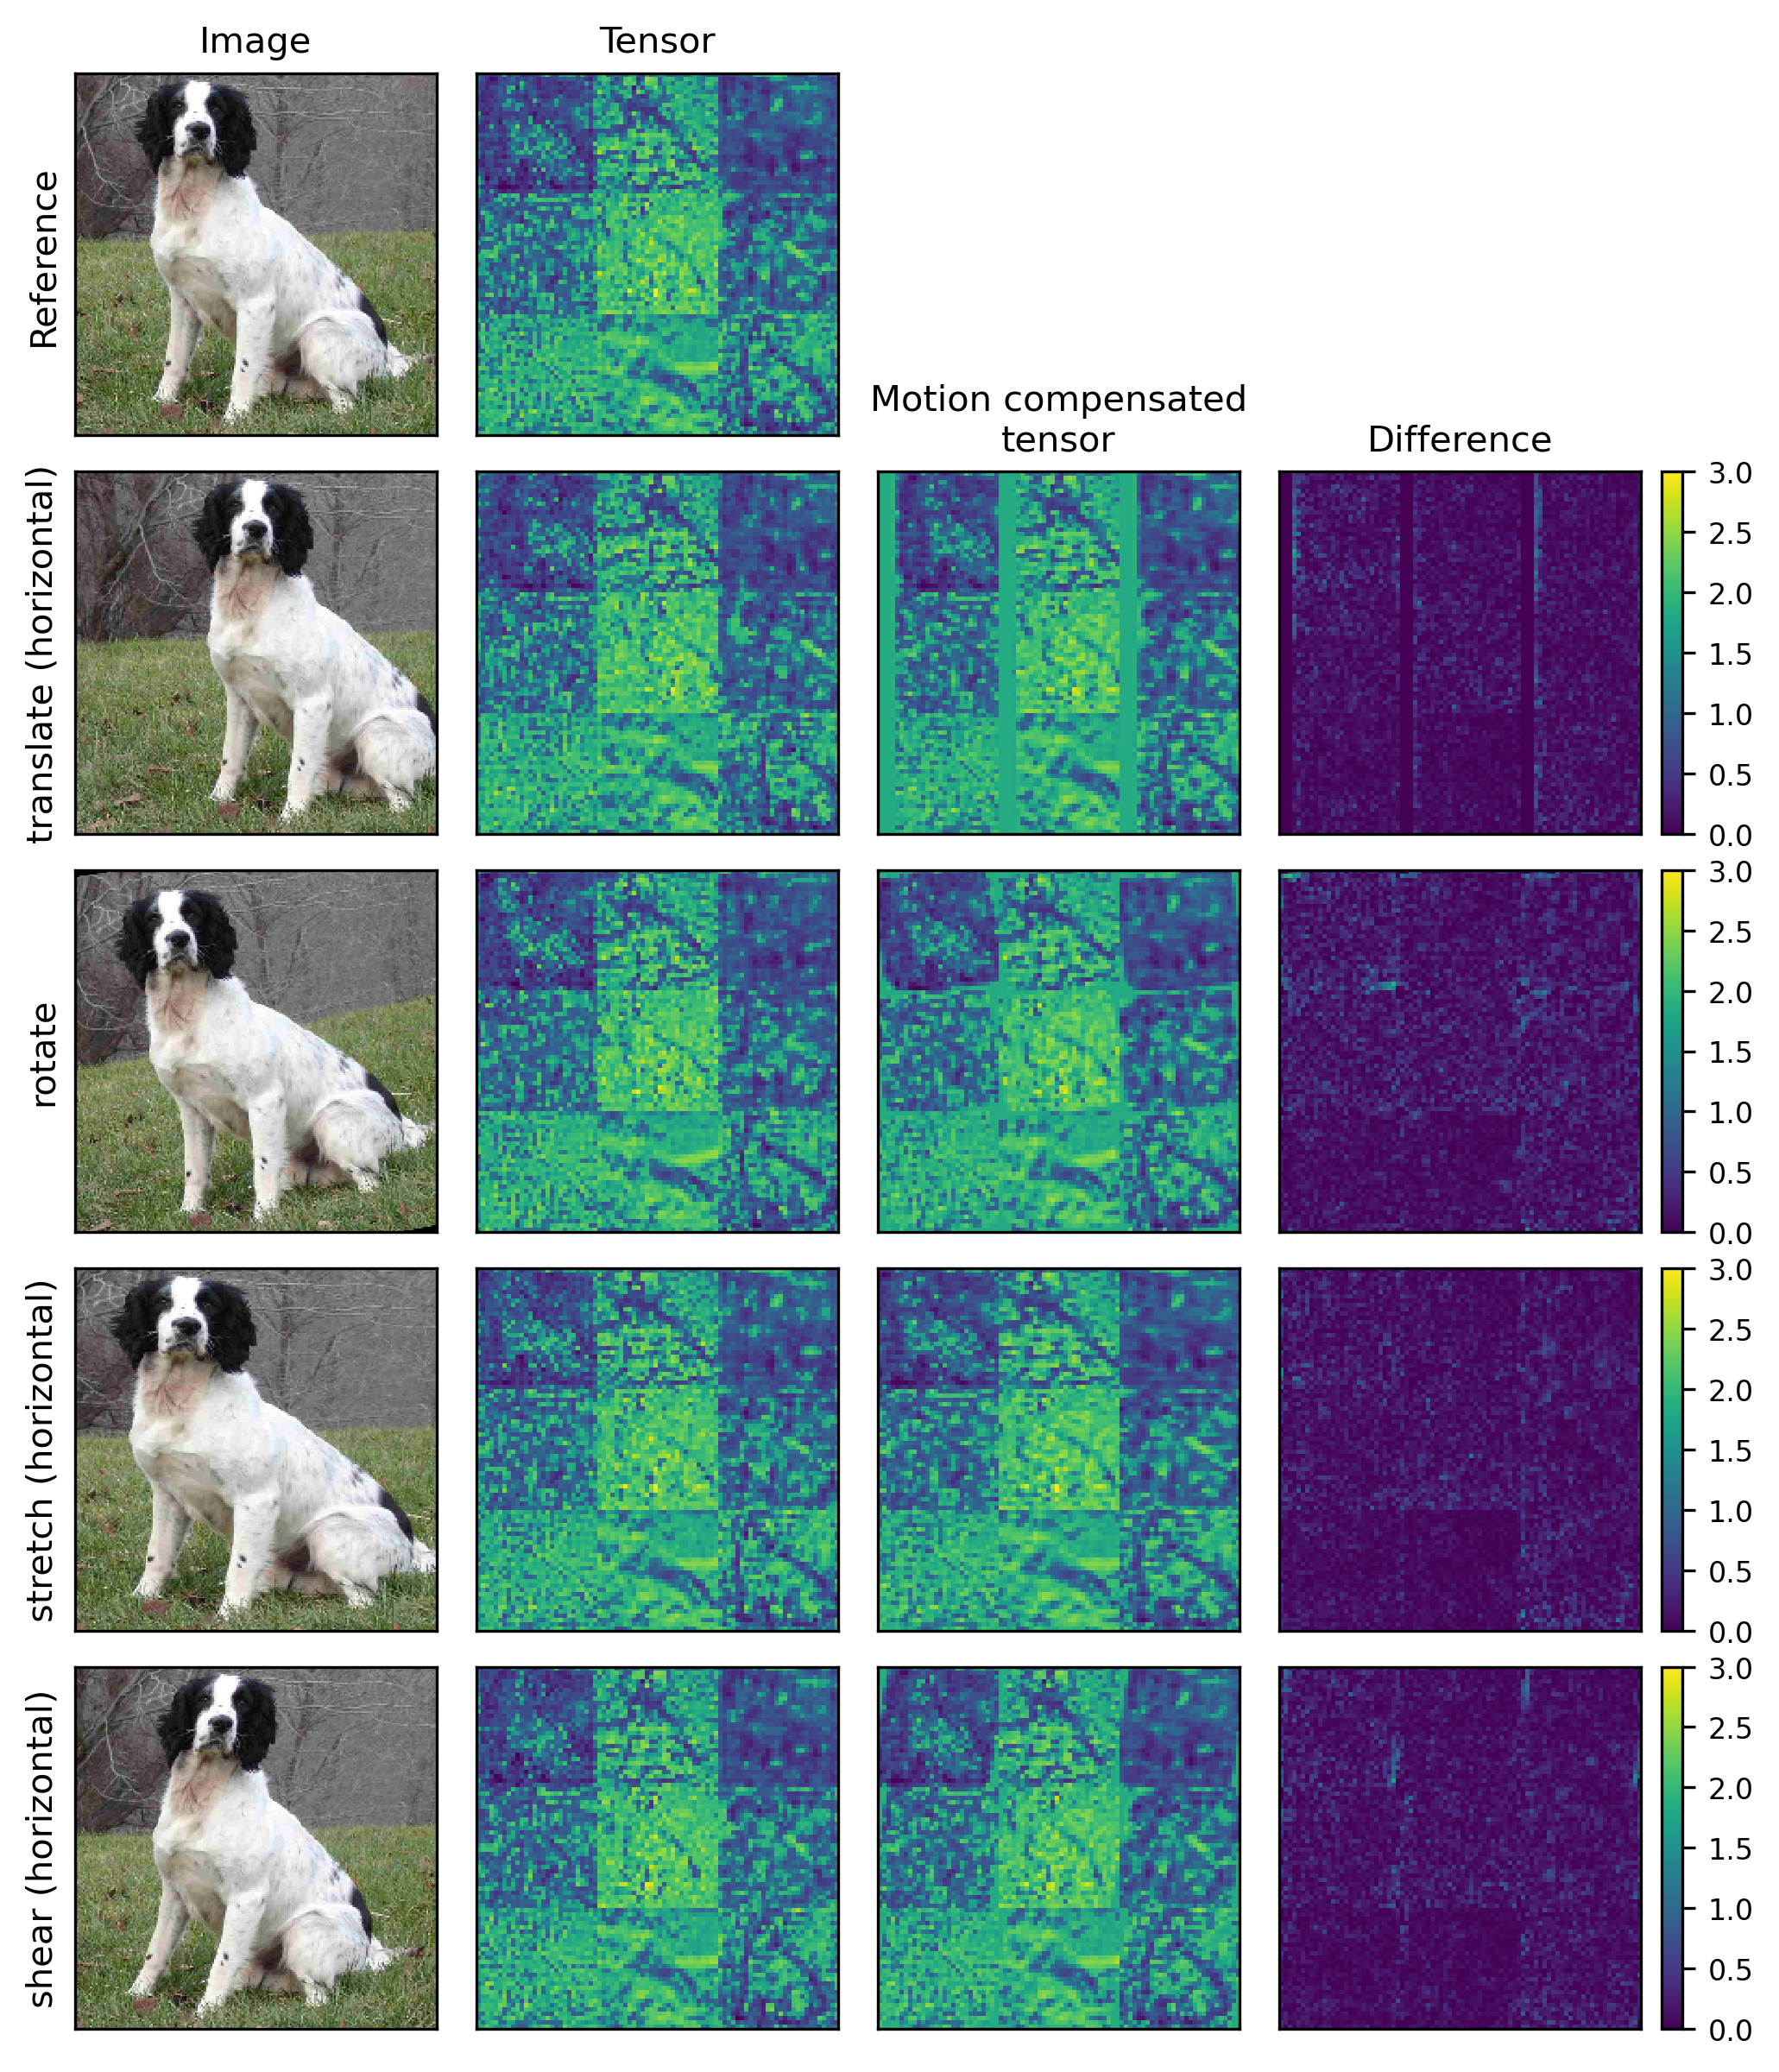
\includegraphics[width=0.95\linewidth]{img/video_latent_space_motion_analysis/examples.png}
    \caption{%
        Examples of motion transformations applied to reference image.
        The output tensors of ResNet-34's add\_3 layer are reliably predicted from only the reference tensor and known input-space motion. % within the pairs of input frames.
        %
        % COLUMNS
        % 1. frame
        % 2. contains "ground truth" tensors computed directly from frame
        % 3. contains predictions
        % 4. is (absolute) difference between third and second
        %
        % ROWS
        % 1. reference
        % 2. horizontal translate by 35 pixels
        % 3. rotate by 10 degrees
        % 4. horizontal scale by 1.2
        % 5. horizontal shear by 10 degrees
    }
    \label{fig:video_latent_space_motion_analysis/examples}
    % \vspace{-1.0\baselineskip}
\end{figure}


%Varied affine transformation parameters for ResNet-34 and DenseNet-121

%In the case of an affine transformation, ...



For quantitative evaluation, experiments were conducted on several layers of ResNet-34~\cite{ResNet} and DenseNet-121~\cite{DenseNet}. Normalized Root Mean Square Error (NRMSE)~\cite{wiki:NRMSE} was used for this purpose:
% \vspace{-7pt}
\begin{equation}
    \text{NRMSE} =  \frac{1}{R} \sqrt{\frac{1}{N} \sum_{i=1}^N (p_i - a_i)^2},
    \label{eq:video_latent_space_motion_analysis/NRMSE}
\end{equation}
where $a_i$ is the actual tensor value produced %by the front end of the DNN
from the transformed input, $p_i$
is the tensor value predicted using our motion model~\cref{eq:video_latent_space_motion_analysis/mv_scale}, $N$ is the number of elements in the feature tensor, and $R$ is the dynamic range. Again, regions that cannot be predicted were excluded from NRMSE computation. \cref{fig:video_latent_space_motion_analysis/transform} shows NRMSE computed across a range of parameters for several transformations, at various layers of the two DNNs. %The brackets in the legends indicate the layer index in the DNN, for example (4/37) means 4$^\text{th}$ out of 37 layers.


\begin{figure*}[tb]
    \centering
    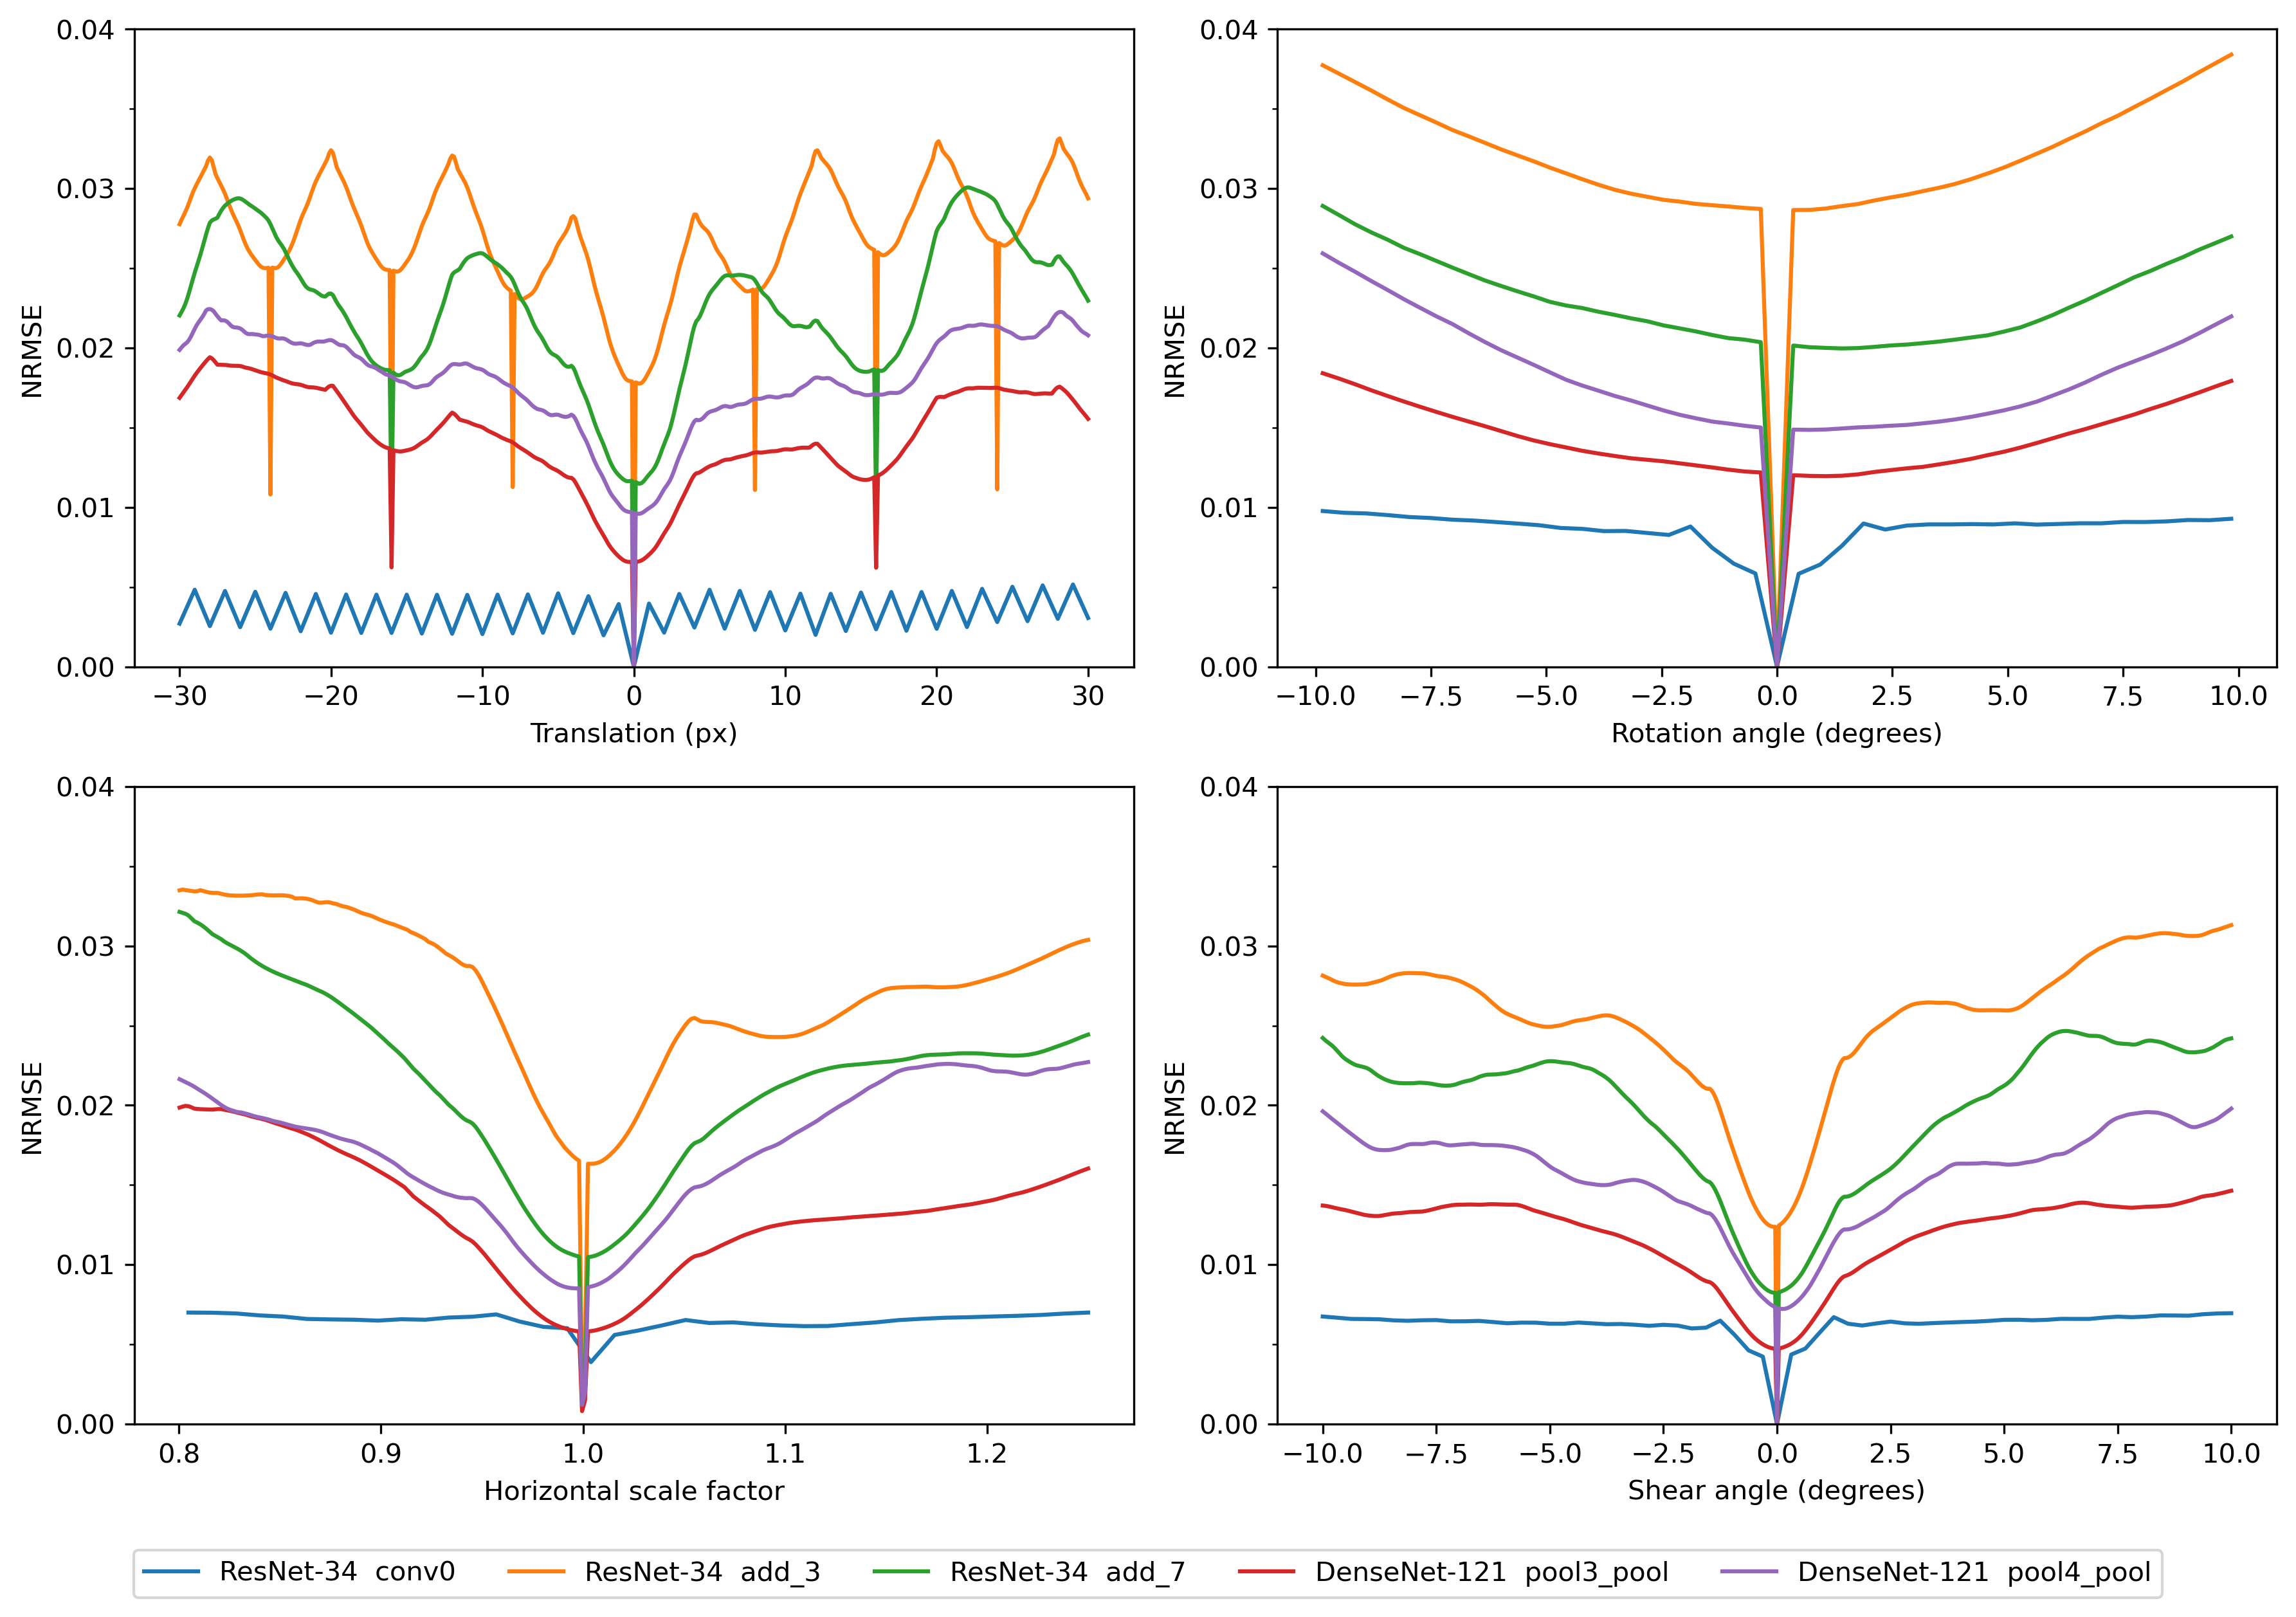
\includegraphics[width=\linewidth]{img/video_latent_space_motion_analysis/nrmse/transform_curves-all.png}
    \caption{%
        NRMSE across parameter ranges for translation (top-left), rotation (top-right), scaling (bottom-left), and shear (bottom-right).
        For translation, NRMSE local minima occur when the input-space shifts correspond to integer latent-space shifts in~\cref{eq:video_latent_space_motion_analysis/mv_scale}.%
    }
    \label{fig:video_latent_space_motion_analysis/transform}
%    \vspace{-10pt}
\end{figure*}



%$R$ is computed from dynamic range of tensor

%after masking out the "non-transformable regions"




%Determine threshold value for what a "typical" codec would see for NRMSE block based matching in typical situation




%The other curves have different periods for translation

As seen in \cref{fig:video_latent_space_motion_analysis/transform}, NRMSE goes up to about 0.04 for reasonable ranges of transformation parameters. How good is this? To answer this question, we set out to find the typical values of NRMSE found in conventional motion-compensated frame prediction.
In a recent study~\cite{Choi_TCSVT_2020}, the quality of frames predicted by conventional motion estimation and motion compensation (MEMC) in High Efficiency Video Coding (HEVC)~\cite{H.265} was compared against a DNN developed for frame prediction. From Table~III in~\cite{Choi_TCSVT_2020}, the luminance Peak Signal to Noise Ratio (PSNR) of frames predicted uni-directionally by the DNN and conventional HEVC MEMC was in the range 27--41 dB over several HEVC test sequences. NRMSE can be computed from PSNR as
% \vspace{-2pt}
\begin{equation}
    \text{NRMSE} = \frac{1}{256}\sqrt{\frac{255^2}{10^{\text{PSNR}/10}}},
% \vspace{-2pt}
\end{equation}
so the PSNR range of 27--41 dB corresponds to the NRMSE range of 0.009--0.044. These levels of NRMSE are indicative of how much motion models used in video coding deviate from the true motion. As seen in \cref{fig:video_latent_space_motion_analysis/transform}, the model~\cref{eq:video_latent_space_motion_analysis/mv_scale} produces NRMSE in the same range, so the accuracy of~\cref{eq:video_latent_space_motion_analysis/mv_scale} is comparable to the accuracy of common motion models used in video coding. Another illustration of this is presented in \cref{fig:video_latent_space_motion_analysis/mse/histogram}, which shows the histogram of NRMSE computed across a range of affine transformation parameters.  Hence,~\cref{eq:video_latent_space_motion_analysis/mv_scale} represents a good starting point for development of latent-space motion compensation.

\begin{figure}[htbp]
    \centering
    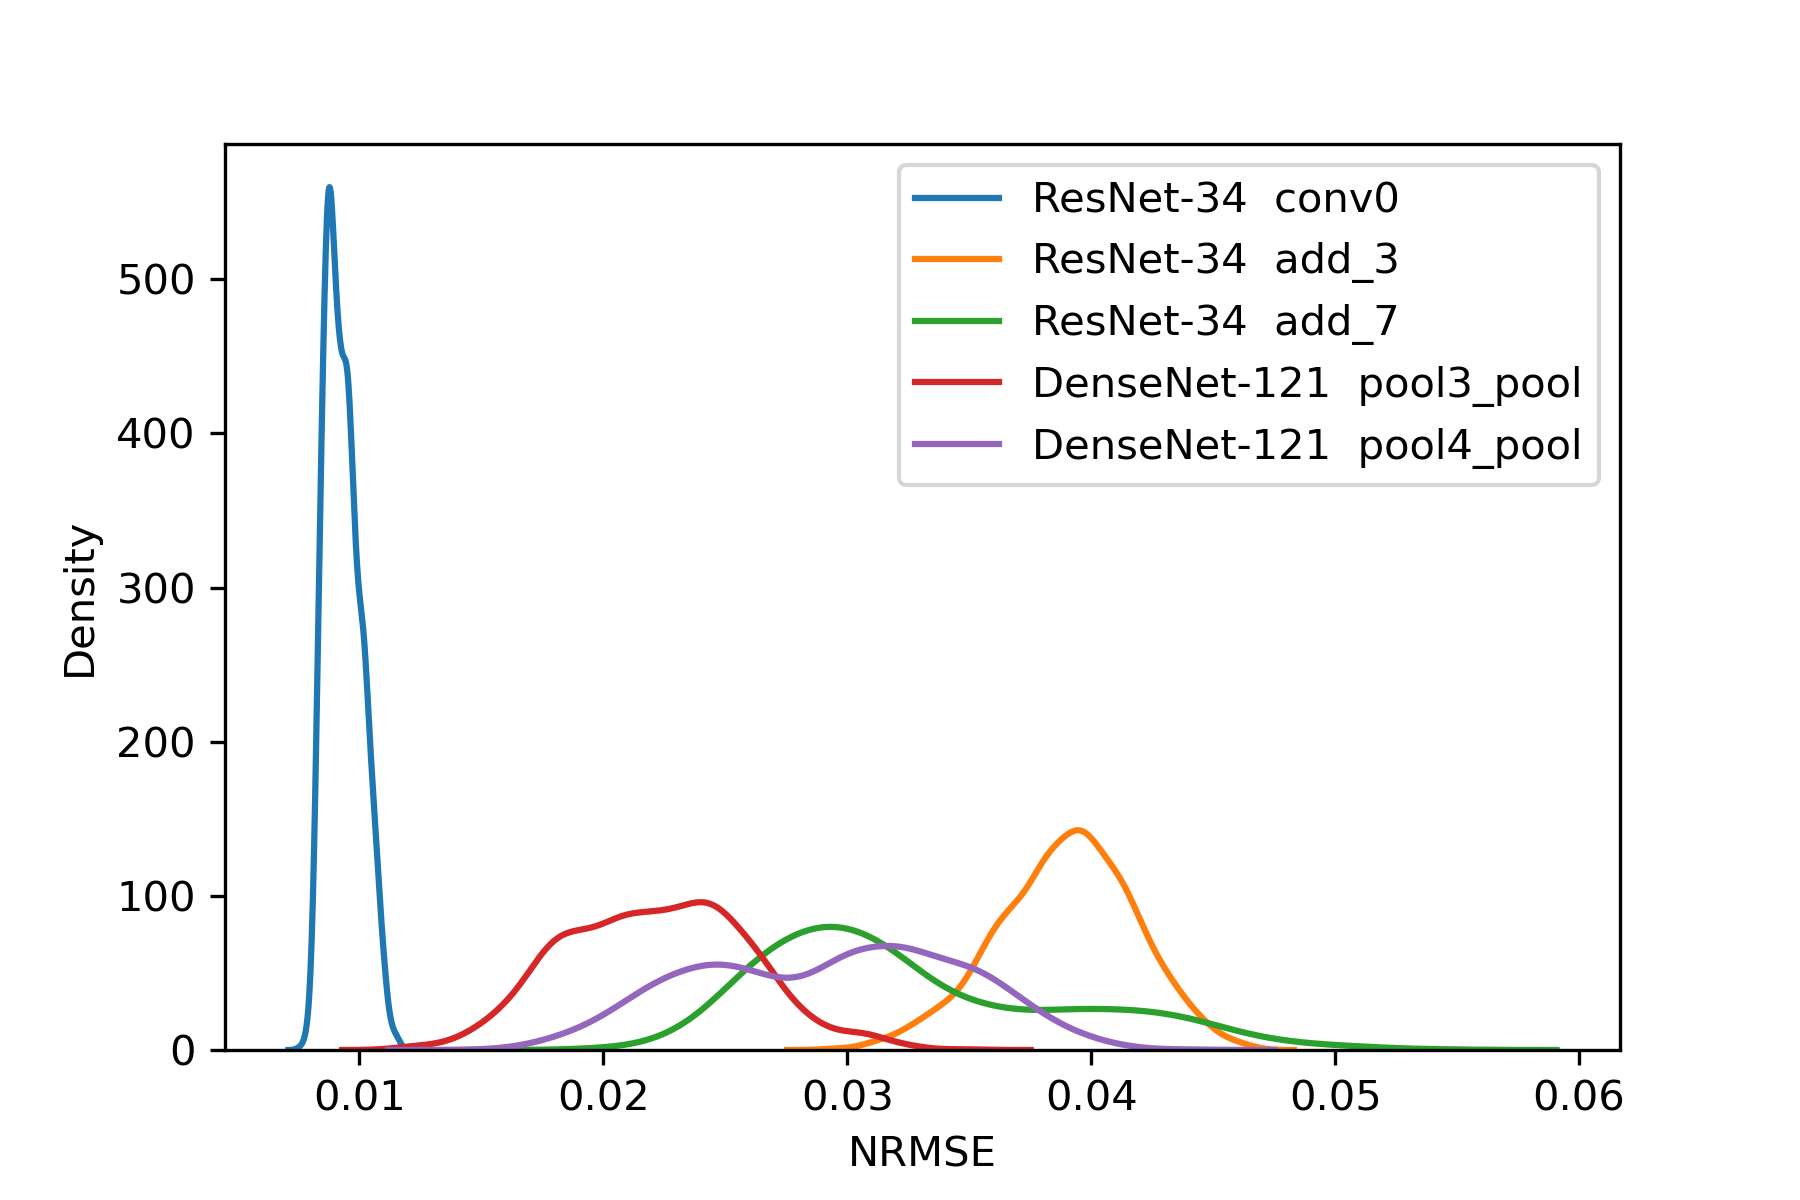
\includegraphics[width=\linewidth]{img/video_latent_space_motion_analysis/nrmse/random.png}
    \caption{%
        NRMSE histogram computed for an affine motion model~\cite{wang_etal_2002} over the combination of the following seven independent uniformly distributed parameters: x- and y-translation ($\pm 32$ px), x- and y-scaling (0.95--1.05), x- and y-shearing ($\pm 5^{\circ}$), and rotation ($\pm 10^{\circ}$).%
        %These roughly model the motion between successive frames in a video sequence.%
    }
    \label{fig:video_latent_space_motion_analysis/mse/histogram}
\end{figure}




\section{Conclusions}
\label{sec:video_latent_space_motion_analysis/conclusions}
Using the concept of optical flow, in this paper we analyzed motion in the latent space of a deep model induced by the motion in the input space, and showed that motion tends to be approximately preserved in the channels of intermediate feature tensors. These findings suggest that motion estimation, compensation, and analysis methods developed for conventional video signals should be able to provide a good starting point for latent-space motion processing, such as motion-compensated prediction and compression, tracking, action recognition, and other applications.
%Another intriguing prospect, which requires further analysis, is the possibility of inferring input-space motion from latent-space features.


\chapter{Conclusion}

In this thesis, we have explored various aspects of learned compression for images, point clouds, and video.

Our first contribution made in \cref{ch:pdf_compression}, "\nameref{ch:pdf_compression}", proposes a simple low-complexity and yet effective method for dynamically adapting the entropy bottleneck to the input distribution.
The static entropy bottleneck is a common component in many SOTA learned compression models.
However, its proportional bitrate usage is minimal in image compression models, in comparison to the Gaussian conditional component --- though, this is likely because of its non-adaptive nature!
Thus, replacing the static entropy bottleneck with an alternative adaptive entropy bottleneck may lead to a small but consistent boost in performance.
It should be noted that a correct plug-and-play end-to-end training implementation of our dynamic entropy model is still under development.

Nonetheless, when trained on a pretrained model with frozen transform weights, our dynamically adaptive entropy bottleneck showed gains of -6.95\% in BD-rate over a static entropy bottleneck.
Thus, our method provides a low-complexity mechanism that can be used to aid in building practical, efficient models for the real world.
Currently, many SOTA models have been largely focused on RD performance.
While the exceptional results on the frontier of RD performance achievement are exciting, it is important to step back and think about how to make learned compression a feasible option for practical use.
Our proposed method takes a step in that direction.
It is quite possible that a practical standardized learned codec might someday make use of our highly efficient low-cost solution in lieu of a heavier alternative.

Our work presented in \cref{ch:point_cloud_compression}, "\nameref{ch:point_cloud_compression}", opens the way for point cloud-oriented machine-task oriented codecs.
We showed how a simple Point Net-based codec focused on the machine task can achieve significantly better results than a more conventional "compress, transmit, decompress, machine task model" approach.
Furthermore, our "micro" encoder operates at an ultra-low complexity of 48 MACs/pt, and yet achieves a far better accuracy for any given bitrate than the conventional approach.

Interestingly, our codec comes close to the theoretical limits of compression for 40 evenly-distributed class labels.
This can in part be attributed to the inherently low entropy of small point clouds.
(e.g. SOTA codecs compress to \~1 bit/pt with acceptable amounts of distortion.)
But another dominant factor is that arguably, the ModelNet40 dataset contains fairly easy-to-classify CAD object point clouds that are noise-free, isolated, and well-defined from all angles.
In comparison, real world point clouds are much noisier, contain a surrounding environment, and often only have measurements visible from a particular angle.
This is evident in the case of LIDAR-generated point clouds.
It is harder to isolate the relevant information in such a setting.
Thus, real-world scenarios present a greater challenge for machine-task oriented codecs.
Nonetheless, we believe that with some effort, machine-task codecs can demonstrate their utility in more complex settings.

In \cref{ch:video_latent_space_motion_analysis}, "\nameref{ch:video_latent_space_motion_analysis}", we showed that in convolutional-based models, motion within the input domain leads to predictable motion within the latent domain.
Furthermore, we quantified how predictable the next "latent frame" is in terms of the amount of residual error that is produced by warping the "reference latent frame".
This is akin to video coding via p-frames, except in the latent domain.
We found that the residual NRMSE is kept under 0.04 for randomly tested "reasonably expected" affine transformations/warps.
(For reference, a NRMSE of 0.04 very roughly corresponds to 27 dB PSNR for conventional image coding.)

Our results suggest that learned video compression approaches that rely upon warping of the latent space are feasible.
Methods such as Scale-Space Flow~\cite{agustsson2020scalespaceflow} rely upon transforming the predicted frame back into the input domain before applying motion-based warping, and then computing the residual frame, and then transforming the residual back into a latent domain for encoding.
Potentially, this costly and possibly even suboptimal step of converting back-and-forth between domains can be eliminated by simply warping the latent space directly, as our study indicates may be viable.

All in all, we believe that our work has contributed to the new and promising field of learned compression.


\backmatter

\clearpage
\phantomsection
\addcontentsline{toc}{chapter}{References}
\printbibliography[title=References]

% \appendix
% \input{tex/appendix.tex}

\end{document}
